\documentclass[UTF8]{article}
% 中文支持
\usepackage[UTF8]{ctex}	
% pdf调用 封面
\usepackage{pdfpages}
% color宏包
\usepackage{color}  
% 导入图片
\usepackage{caption}
\usepackage{graphicx, subfig}
% 防止图片乱跑
\usepackage{float}
% 支持数学符号
\usepackage{amsmath}
% 支持代码块
\usepackage{listings}
% pdf加入大纲
\usepackage{hyperref}
% 大纲去红框
\hypersetup{hidelinks,
	colorlinks=true,
	allcolors=black,
	pdfstartview=Fit,
	breaklinks=true
}

% 绘制三线表
\usepackage{booktabs}    
% 消除警告
\usepackage{lmodern}

% 绘图
\usepackage{tikz}
\usetikzlibrary{positioning, shapes.geometric}
\tikzstyle{bag} = [align=center]

% 设置页面的环境,a4纸张大小,左右上下边距信息
\usepackage[a4paper, left=31.8mm, right=31.8mm, top=25.4mm, bottom=25.4mm]{geometry}

% 代码块的基本设置
\lstset{
 breaklines,%自动换行
 columns=fixed,       
 numbers=left,                                        % 在左侧显示行号
 numberstyle=\tiny\color{gray},                       % 设定行号格式
 frame=none,                                          % 不显示背景边框
 backgroundcolor=\color[RGB]{245,245,244},            % 设定背景颜色
 keywordstyle=\color[RGB]{40,40,255},                 % 设定关键字颜色
 numberstyle=\footnotesize\color{darkgray},           
 commentstyle=\it\color[RGB]{0,96,96},                % 设置代码注释的格式
 stringstyle=\rmfamily\slshape\color[RGB]{128,0,0},   % 设置字符串格式
 showstringspaces=false,                              % 不显示字符串中的空格
 language=python,                                        % 设置语言
}

% \begin{titlepage}
% % 封面信息
% \includepdf[pages={1}]{cover.pdf}
% \end{titlepage}

% 生成目录
% \tableofcontents
% \cleardoublepage

% 导入图片
% \begin{figure}[H]
%     \centering % 居中 
%     % 图片文件的相对路径
%     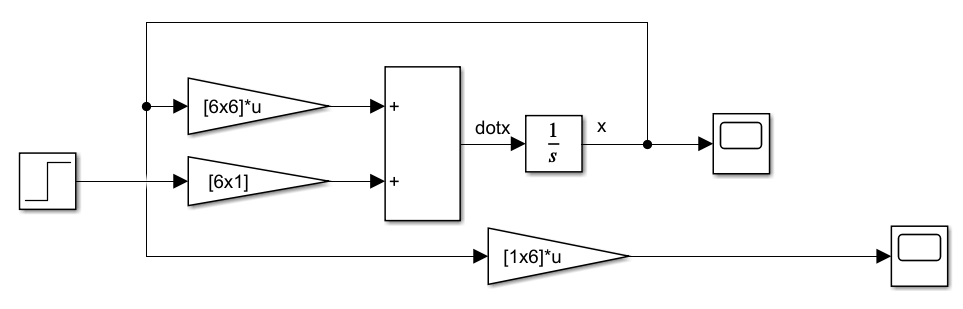
\includegraphics[width=.8\textwidth]{figure/exp1_1_model.png} 
%     \caption{Simulink模型} % caption是图片的标题
%     % \label{img} % 此处的label相当于一个图片的专属标志,目的是方便上下文的引用
% \end{figure}

% 导入代码
% \begin{lstlisting}
% a
% \end{lstlisting}

\begin{document}

% 报告名称要与课程名称一致!!

% 封面:应包含有正确的课程名称、姓名、小组序号、开展实习的年份这些基本信息。
% 报告名称务必与课程名称一致,不得任意起名。内容包含但不限于:
% (1)实习目标和任务简述
% (2)控制系统简介:含对象+控制器+各类仪表
% (3)控制系统设计及运行结果: 各类控制策略的实习过程及运行结果(可以分小节)。
% (4)实习心得与体会
% 注意:格式规范(含层次)、图文并茂(需要图名和图号)、语句通顺(第三人称论述)、逻辑清晰、文献引用规范。

% 内容要求:
% 1. 画出PI\&D(管道工艺流程图)方案(需要进行综合分析,选取较好的控制方式)
% 2. 给出程序设计思路
% 3. 给出PID参数调整结果和参数变化曲线图(扰动作用下4:1曲线,要求被控参数和阀门/变频器度曲线一起展示)
% 4. 对象辨识结果,要求在其中1类控制中要有所体现(Matlab中虚拟调试PID结果与实际控制PID结果需要进行对比)

% 自己负责的部分:系统辨识,
% 使用PID模块:单回路,串级,比值控制

\begin{titlepage}
% 封面信息
\includepdf[pages={1}]{./cover/cover.pdf}
\end{titlepage}

% 生成目录
\tableofcontents
\cleardoublepage

%
\section{实习目标、任务简述与分工}
%%
\subsection{实习目标}
本次过程控制综合实践I: PLC-DCS 综合设计实习课程以现代过程控制原理与应用技术为基础,运用PLC(可编程逻辑控制器)技术进行DCS(集散控制系统)架构下过程控制系统的设计和集成,完成以案例为设计目标的过程控制系统分析、设计、控制、投运。主要包括:过程控制系统工艺分析、过程控制系统方案设计、过程检测和执行通道配置、PLC控制程序设计、系统参数整定和投运。通过实践教学,达到学生在借助现代先进控制工具和软件基础上,能灵活运用《现代过程控制原理与应用技术》理论知识在DCS框架下运用现代化工具PLC进行复杂过程对象的控制系统设计,培养学生解决复杂控制问题的能力。同时培养学生在工程实践中的沟通、团队协作和项目管理能力,并考虑具体实施中的安全、健康、法律、文化和环境等因素约束条件;拓宽学生的知识面,培养学生分析问题、解决问题的能力,启动学生的创造性思维。
具体课程目标如下:
\begin{enumerate}
	\item 了解案例问题的系统组成、控制需求、控制任务、控制工艺以及将要实施的控制系和技术的先进性情况;
	\item 能灵活综合运用所学知识,在自学PLC技术基础上开展控制系统的系统建模、控制工艺分析和控制方案设计与讨论,培养具备依据控制需求确定最佳工程实施方案和技术路线的能力;
	\item 培养具备运用PLC技术进行DCS结构下复杂过程控制系统的设计及投运的能力,并完成具体实施工作,如控制策略选取、系统搭建、软件设计、系统投运;
	\item 掌握DCS系统下过程控制系统设计、集成、投运的一般步骤和方法,培养具备PID单回路控和复杂控制系统的控制程序开发,参数整定和系统投运,过程检测和控制通道调校,安全连锁设计,DCS系统下控制系统工程实施的能力;
	\item 充分发挥团队协作能力开展复杂控制任务的分解和协同工作,在考虑解决方案对社会、健康、安全、法律以及文化的影响基础上进行不断分析、评判和优化,具备利用PLC技术构建集散系统,并具有考虑非技术因素下的对系统进行全面优化设计的能力。
\end{enumerate}

%%
\subsection{任务简述}
以实验室水箱实验装置为实验对象,PLC 作为现场控制站控制单元,触摸屏作为现场操作监控单元,构建基于 PLC 的 DCS 单站(多站)系统。开展涉及如下内容的设计工作:
\begin{enumerate}
	\item 系统结构组成与电气原理认识,含水路流通管路、传感器和执行器特性和性能、接线理图;
	\item 完成1类被控对象的测试和模型辨识(必做),可以选择单容水箱、双容水箱、并列水箱、阀门、管路等对象开展系统辨识;可以PLC提取数据,Matlab中进行模型辨识,给出被控对象的传递函数。
	\item 开展任意参数的单回路(必做)(压力、流量、液位),串级(必做)(液位-压力、液位-流量、流量-压力、),前馈-反馈、比值、解构控制,即小组自选控制参数、自选控制策略。要求:1-画出PI\&D(管道工艺流程图)方案(需要进行综合分析,选取较好的控制方式)、2-给出程序设计思路、3-给出PID参数调整结果和参数变化曲线图(扰动作用下4:1曲线,要求被控参数和阀门/变频器度曲线一起展示)。5-其中(2)中的对象辨识结果,要求在其中1类控制中要有所体现(Matlab中虚拟调试PID结果与实际控制PID结果需要进行对比)。控制系统设计中需要团队协作和沟通,组织肩负项目管理作用。
	\item 系统辨识、单回路和串级必须完成(只完成该部分的,成绩合格或中等),完成前者基础上再增加1-2种控制,依据控制性能情况(成绩良好或优秀)。以上控制中,需要:1-在一个完整的软件程序项目中完成(需要利用系统进行多回路同时控制或受制于设备可分阶段控制,不能多次下载控制程序进行单独项目控制,但可通过控制切换实现);2- 具备手动与自动控制能力,手动即直接操作阀门/变频器控制,自动化即PID控制(手自动切换中,尽量采取无扰切换方式)。注意:算法不限于PLC库中的PID,可以自己写算法(人工智能,控制算法)。
	\item 给出简单图形界面(美观性不作为验收依据,功能性作为验收依据)。HMI没有统一要求,自行设计。(曲线显示可以在界面中显示,也可以导出数据在matlab中绘制)
\end{enumerate}

%%
\subsection{个人分工}
在本次实习中,我主要负责如下部分:
\begin{itemize}
    \item PLC与计算机的网络通讯
	\item 基于水箱液位的系统参数辨识
	\item 主水箱液位单回路控制系统设计(基于PID模块)
	\item 主水箱液位-流量串级控制系统设计(基于PID模块)
	\item 主副水箱液位比值控制系统设计
\end{itemize}

由于以上的控制系统设计中部分控制系统分别使用了博图软件中的PID模块和自行设计的PID算法程序,故小组成员之间的分工内容互有重叠。

%
\section{控制系统简介}
% 控制对象:水箱
% - 系统结构组成
%   - 水路流通管路
%   - 各类传感器 特性 性能
%   - 执行器
%     - 电磁阀(工频泵)
% 	- 变频泵
% - 接线理图

%%
\subsection{实习所用设备介绍}

本次PLC实习所用的主要设备有:
西门子S7-1200可编程逻辑控制器件,搭配各种辅助设备如交换机、台达显示屏(触摸屏),电源等。

西门子水箱实验台,包含了主、副两个水箱、一个变频器和变频电机、一个工频电机、一个电磁阀、两个液位变送器、两个流量变送器、两个压力变送器,以及若干手动阀。

此外,还需要一台安装有博图软件(建议v15.1以上)的带有网口或配备USB扩展网口的计算机。

%%
\subsection{系统DCS架构介绍}
DCS(Distributed Control System)即集散控制系统,主要由集中操作与管理系统、分散控制单元,以及通信系统组成。基于DCS的控制系统架构,使其能够实现对工业过程的高效、可靠和自动化的控制。下面是集散控制系统的简单示意图:
\begin{figure}[H]
    \centering % 居中 
    % 图片文件的相对路径
    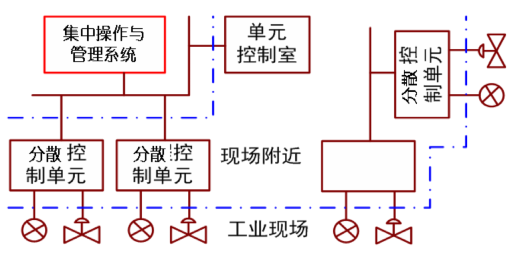
\includegraphics[width=.6\textwidth]{figure/DCS示意图.png} 
    \caption{集散控制系统示意图} % caption是图片的标题
    % \label{img} % 此处的label相当于一个图片的专属标志,目的是方便上下文的引用
\end{figure}

在本次实习中,可以粗略地认为水箱实验台和西门子PLC现场控制单元共同组成了一个集散控制系统中的一个分散控制单元。在一个完整的集散控制系统中,集中操作与管理系统通常包括人机交互设备,供操作员对工业过程进行监视和在必要的时候下发控制指令;分散控制单元通常基于微控制器构建,主要负责对现场的各种工业过程进行监视和实现独立的闭环控制;通信系统通常包括现场总线、工业以太网等,是分散控制单元和集中操作管理系统的连接桥梁,负责对各种信号进行实时传输。结合我们实习所使用的设备,可以将PLC和水箱实验台看做对水箱系统所涉及到的过程进行控制的一个分散控制单元。


%%
\subsection{系统结构组成与电气原理}
%%%
\subsubsection{水箱实验台}
本次实习中以水箱实验台作为实验对象,包含了主副两个水箱,每个水箱均有单独的出水阀门和进水管道;实验台提供了工频泵和变频泵用来向水箱供水,且每个泵都可以通过设置相应的手动阀来决定向哪个水箱供水;除此之外,实验台还提供了多种传感器用于检测水箱系统运行过程中的各种数据,这些传感器包括用来检测主副水箱液位的液位变送器,检测工频段和变频段水流管道流量的流量变送器,以及负责检测压力的压力变送器(本次实习中未用到)等。

水箱实验台实物结构图如下所示:
\begin{figure}[H]
    \centering % 居中 
    % 图片文件的相对路径
    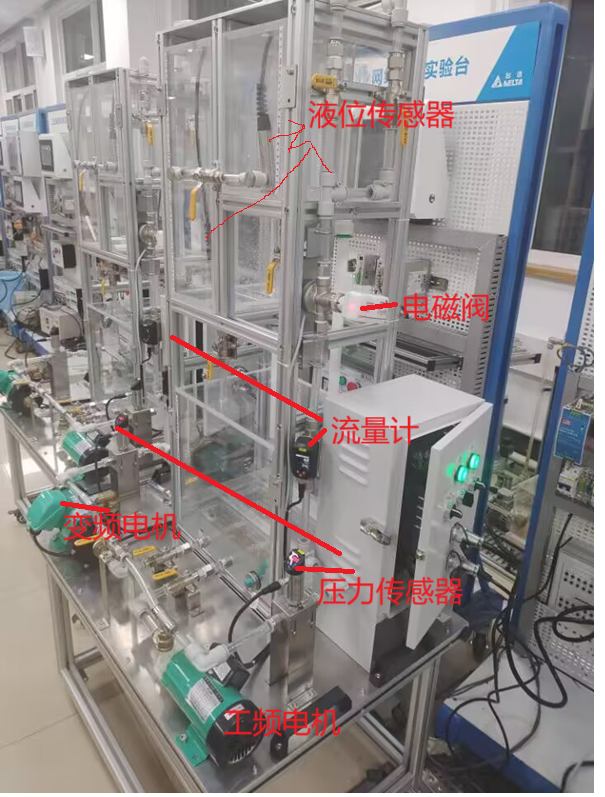
\includegraphics[width=.6\textwidth]{figure/水箱实验台实物结构图.png} 
    \caption{水箱实验台实物结构图} % caption是图片的标题
    % \label{img} % 此处的label相当于一个图片的专属标志,目的是方便上下文的引用
\end{figure}

%%%
\subsubsection{PLC现场控制单元}
本次实习使用西门子S7-1200 PLC作为水箱系统的现场控制单元,搭配了对应的西门子输入/输出IO模块,在博图软件中配置其设备组态如下图所示:
\begin{figure}[H]
    \centering % 居中 
    % 图片文件的相对路径
    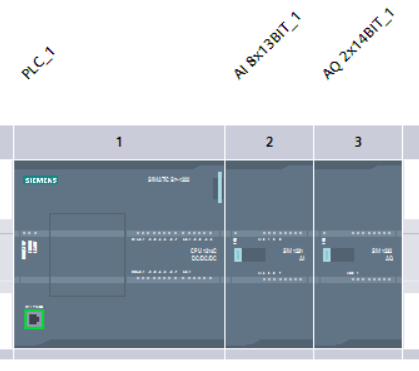
\includegraphics[width=.6\textwidth]{figure/PLC设备组态.png} 
    \caption{PLC设备组态} % caption是图片的标题
    % \label{img} % 此处的label相当于一个图片的专属标志,目的是方便上下文的引用
\end{figure}

由于实习中不同水箱设备的各种信号接口与PLC连接端口的连接情况并不完全一致,这里仅列出各种信号接口的连接IO类型,如下表所示:
\begin{table}[H] % 防止表格乱跑
\centering % 居中
\begin{tabular}{ccc} % 指明列数
	\toprule % 顶部粗线
	所用设备 & 传输信号 & 对应PLC接口类型 \\
	\midrule % 中间细线
	工频段流量变送器 & 工频段流量计流量 & AI \\ 
	变频段流量变送器 & 变频段流量计流量 & AI \\ 
	工频段水管压力变送器 & 工频段水管压力 & AI \\ 
	变频段水管压力变送器 & 变频段水管压力 & AI \\ 
	主水箱液位变送器 & 主水箱液位 & AI \\
	副水箱液位变送器 & 副水箱液位 & AI \\
	变频器 & 变频器频率反馈 & AI \\
	变频泵(变频器) & 变频电机工作频率 & AQ \\
	电磁阀 & 电磁阀开度 & AQ \\
	\bottomrule % 底部粗线
\end{tabular}
\caption{PLC与水箱设备信号接口} % 标题
\end{table}
其中AI表示模拟量输入,AQ表示模拟量输出。

%
\section{基于单容水箱液位的系统模型辨识}
%%
\subsection{对象特性分析}
根据在过程控制课程上所学的内容可以知道,单容水箱为一阶对象。因此可以采用阶跃响应曲线法对该一阶系统的参数进行辨识。
\begin{figure}[H]
    \centering % 居中 
    % 图片文件的相对路径
    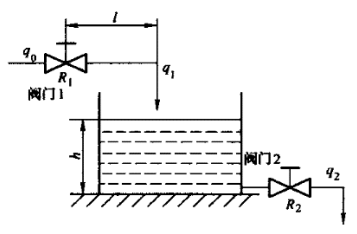
\includegraphics[width=.6\textwidth]{figure/单容水箱模型.png} 
    \caption{单容水箱模型} % caption是图片的标题
    % \label{img} % 此处的label相当于一个图片的专属标志,目的是方便上下文的引用
\end{figure}

%%
\subsection{辨识数据采集}
基于变频泵为主水箱供水,主水箱出水口的阀门保持一定开度,使用简单的PID闭环控制将主水箱液位控制在20cm高度处并保持稳定,读取此时的变频泵输入给定值并记录。将闭环控制改为手动开环控制方式,然后将变频泵的输入改为上述记录的给定值,使得主水箱液位在开环控制方式下稳定在20cm高度处。

待主水箱液位稳定后,对变频泵输入一个阶跃信号,即将变频泵输入给定值增大,由于水箱是一个自衡系统,这时主水箱液位将会逐渐自衡到新的高度。在这一过程中,使用PLC以固定的采样时间0.3s记录主水箱的液位数据,并导出至MATLAB中进行分析。

%%
\subsection{基于MATLAB系统辨识工具箱进行水箱系统辨识}
通过理论分析可以知道,单容水箱通常是一个无滞后的一阶对象,其传递函数一般可以表示为:
\begin{equation*}
	G(s) = \frac{K}{Ts + 1}
\end{equation*}

然而,在我们使用的实际水箱系统中,往往会由于水流管道等各种原因导致系统出现一定程度的纯滞后现象。因此,这里将实际单容水箱系统当做一个具有纯滞后的一阶对象,其传递函数可以表示为:
\begin{equation*}
	G(s) = \frac{K\cdot e^{-\tau s}}{Ts + 1}
\end{equation*}

使用MATLAB软件中自带的系统辨识工具箱,对基于上述具有纯滞后的一阶对象传递函数模型进行主水箱系统参数辨识,使用的数据包括水箱液位变化数据以及对应的阶跃信号输入,如下图所示:
\begin{figure}[H]
    \centering % 居中 
    % 图片文件的相对路径
    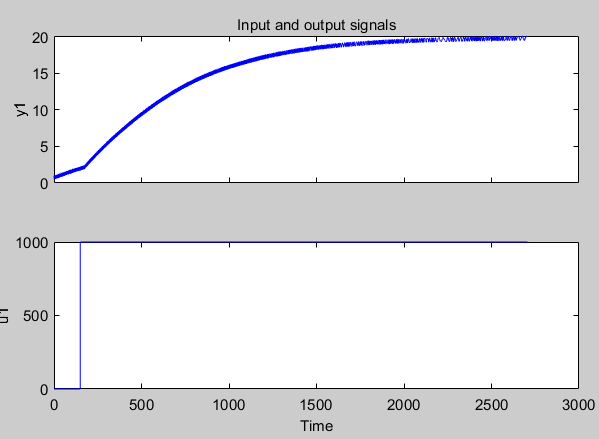
\includegraphics[width=.6\textwidth]{figure/水箱辨识-辨识所用数据.png} 
    \caption{水箱系统辨识所用数据} % caption是图片的标题
    % \label{img} % 此处的label相当于一个图片的专属标志,目的是方便上下文的引用
\end{figure}

%%
\subsection{水箱系统辨识结果}
MATLAB系统辨识工具箱的辨识结果截图如下:
\begin{figure}[H]
    \centering % 居中 
    % 图片文件的相对路径
    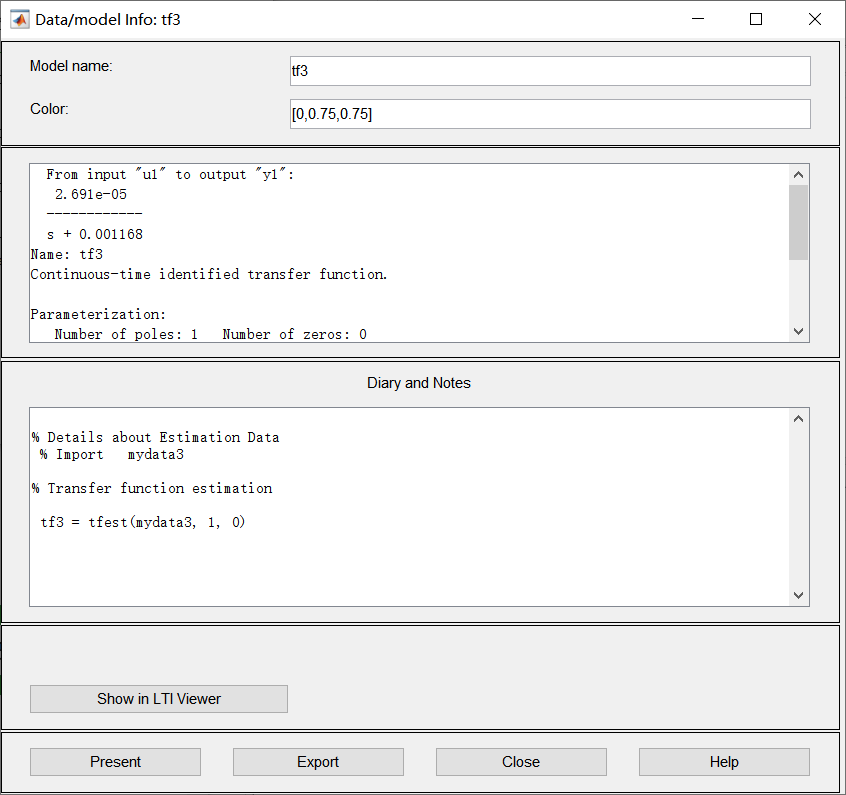
\includegraphics[width=.6\textwidth]{figure/水箱辨识-传递函数.png} 
    \caption{辨识结果截图} % caption是图片的标题
    % \label{img} % 此处的label相当于一个图片的专属标志,目的是方便上下文的引用
\end{figure}

辨识结果的曲线拟合情况如下图所示:
\begin{figure}[H]
    \centering % 居中 
    % 图片文件的相对路径
    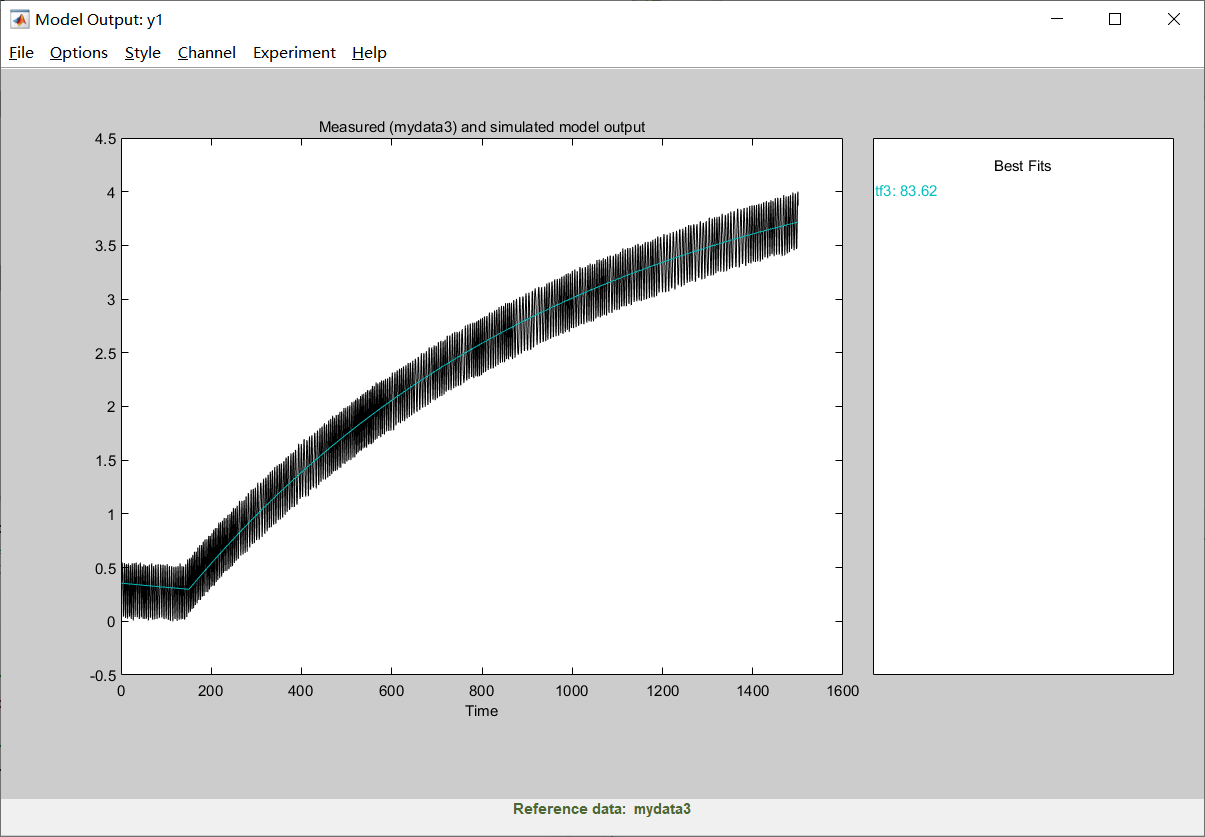
\includegraphics[width=.8\textwidth]{figure/水箱辨识-拟合曲线.png} 
    \caption{辨识结果的曲线拟合情况} % caption是图片的标题
    % \label{img} % 此处的label相当于一个图片的专属标志,目的是方便上下文的引用
\end{figure}

最后得到的单容水箱系统的传递函数模型如下:
\begin{equation*}
	G(s) = \frac{0.02304 \cdot e^{-4.5s}}{856.2s + 1}
\end{equation*}

%%
\subsection{虚拟PID调试}
使用MATLAB软件中的PID调试工具,针对上述单容水箱模型进行PID控制器的调试,最终的控制效果如下图所示:
\begin{figure}[H]
    \centering % 居中 
    % 图片文件的相对路径
    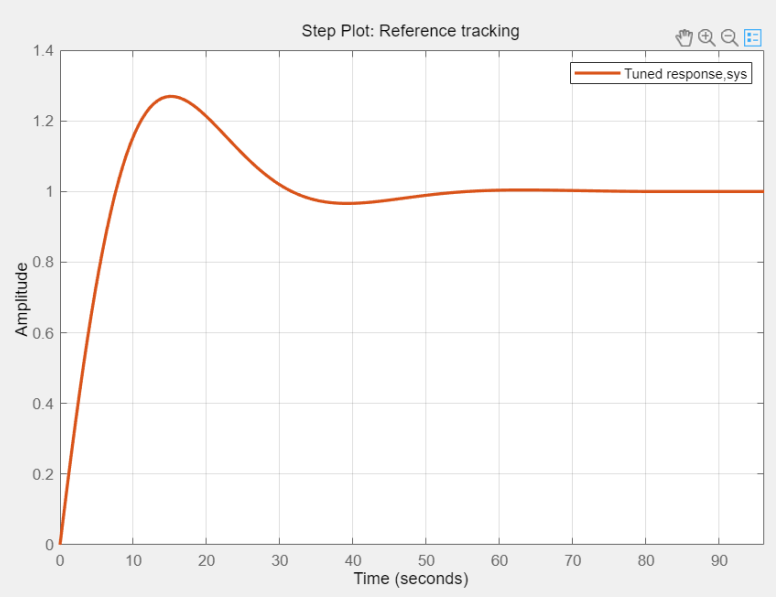
\includegraphics[width=.6\textwidth]{figure/水箱辨识-虚拟pid调试.png} 
    \caption{虚拟PID调试效果图} % caption是图片的标题
    % \label{img} % 此处的label相当于一个图片的专属标志,目的是方便上下文的引用
\end{figure}

%
\section{控制系统设计及运行结果}
%%
\subsection{主水箱液位单回路控制系统设计(基于PID模块)}
%%%
\subsubsection{控制系统设计}
对于单回路控制系统设计,我们选择主水箱作为控制对象,变频泵作为执行器,主水箱液位变送器为检测设备。其中主水箱液位为被控量,变频器工作频率为控制量,并使用PID控制器构成单回路闭环控制系统。主水箱液位控制系统框图如下所示:
\begin{figure}[H]
    \centering % 居中 
    % 图片文件的相对路径
    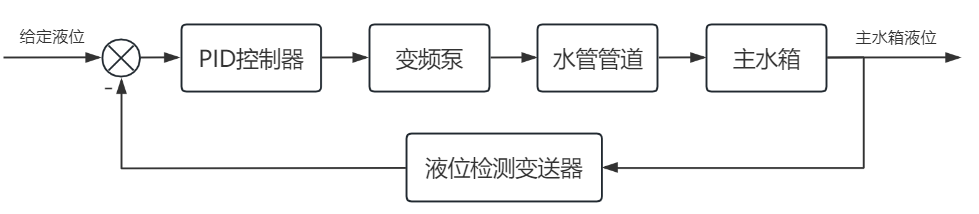
\includegraphics[width=.8\textwidth]{figure/主水箱液位单回路控制系统框图.png} 
    \caption{主水箱液位单回路控制系统框图} % caption是图片的标题
    % \label{img} % 此处的label相当于一个图片的专属标志,目的是方便上下文的引用
\end{figure}

%%%
\subsubsection{程序设计}
采用PLC库中的PID模块构建单回路控制系统的PID控制器部分,其程序设计图如下:
\begin{figure}[H]
    \centering % 居中 
    % 图片文件的相对路径
    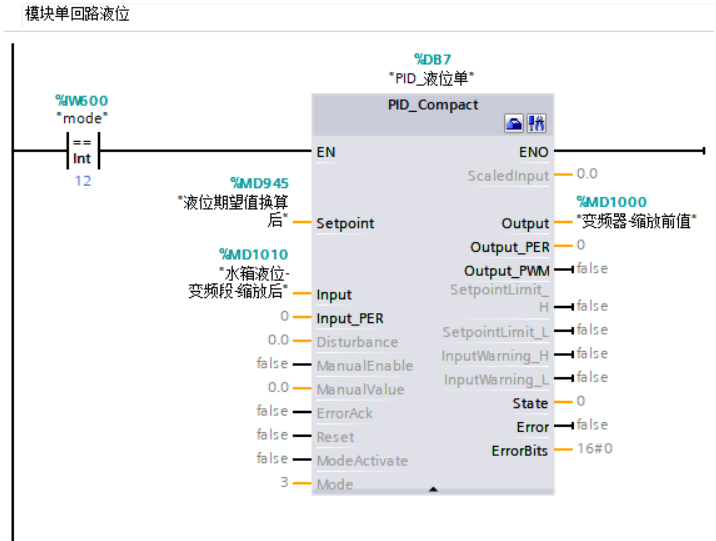
\includegraphics[width=.8\textwidth]{figure/单回路-模块.PNG} 
    \caption{主水箱液位单回路控制系统程序图} % caption是图片的标题
    % \label{img} % 此处的label相当于一个图片的专属标志,目的是方便上下文的引用
\end{figure}

经参数整定后,最终使用的PID控制器各参数如下:
\begin{figure}[H]
    \centering % 居中 
    % 图片文件的相对路径
    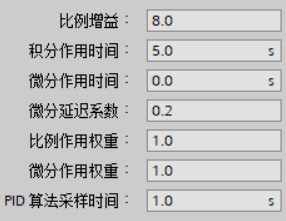
\includegraphics[width=.4\textwidth]{figure/单回路-模块-PID参数.png} 
    \caption{单回路控制器参数} % caption是图片的标题
    % \label{img} % 此处的label相当于一个图片的专属标志,目的是方便上下文的引用
\end{figure}

%%%
\subsubsection{控制效果展示}
主水箱液位单回路控制系统的控制效果如下所示:
\begin{figure}[H]
    \centering % 居中 
    % 图片文件的相对路径
    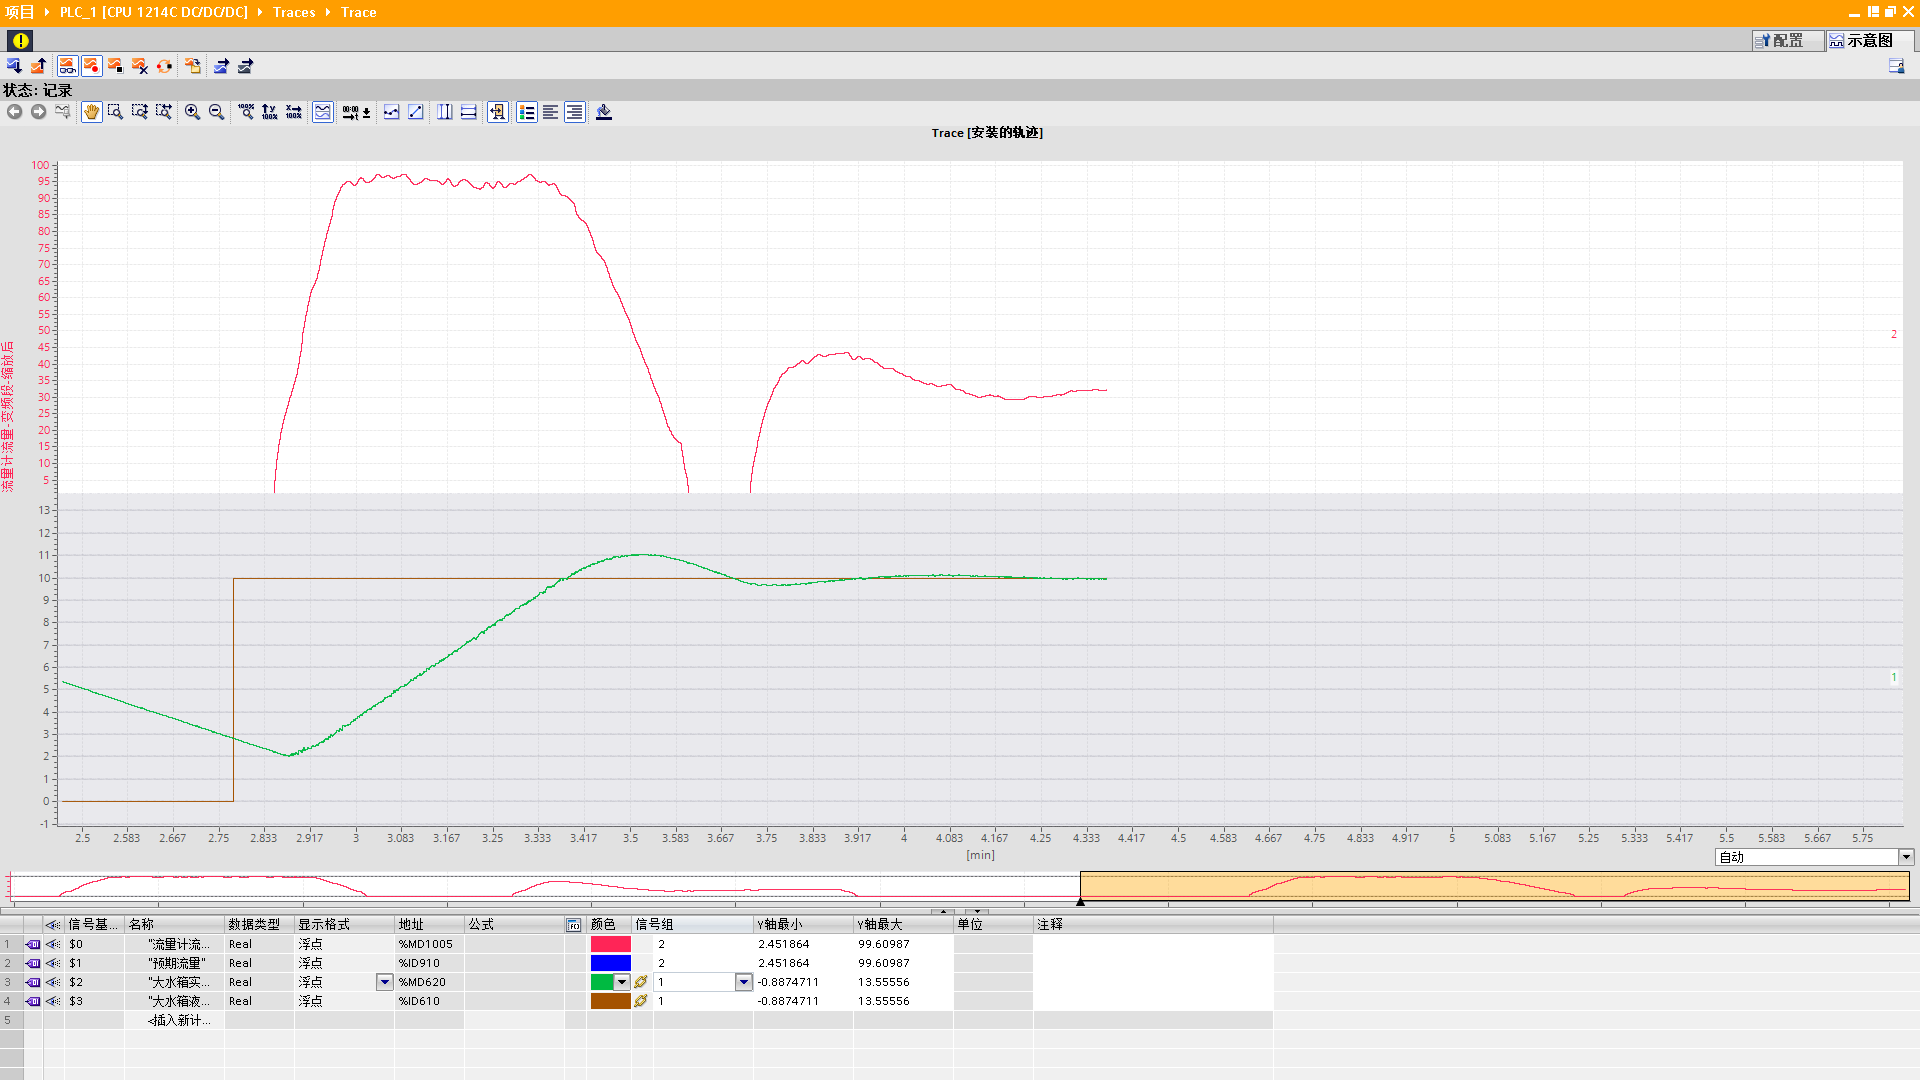
\includegraphics[width=1\textwidth]{figure/单回路控制效果-模块.png} 
    \caption{主水箱液位单回路控制效果} % caption是图片的标题
    % \label{img} % 此处的label相当于一个图片的专属标志,目的是方便上下文的引用
\end{figure}
其中,绿色曲线代表主水箱实际液位,棕色曲线代表主水箱液位给定值,红色曲线代表变频段管道流量值。可以看到,主水箱实际液位的调节曲线出现了幅值比例约4:1的两个波峰,符合控制要求。

%%
\subsection{主水箱液位单回路控制系统设计(基于自行设计的PID)}
%%%
\subsubsection{增量式PID控制器设计}
增量式PID控制器在某些关键方面优于位置式PID,特别是在处理积分饱和问题方面。在位置式PID中,积分项持续累积,尤其在系统误差较大时,可能导致控制器饱和。相比之下,增量式PID通过计算控制量的增量来操作,显著降低了积分饱和的风险。这一点在数字控制系统中尤为重要,因为增量式PID直接计算控制量的变化,更适合于离散时间控制系统,特别是在微处理器控制系统中。因此,在编写自定义的PID控制算法时,我们选择使用增量式PID而非位置式PID。增量式PID的公式如下:
\begin{equation*}
	\Delta u(t) = K_p[e(t) - e(t-1)] + K_ie(t) + K_d[e(t) - 2e(t-1) + e(t-2)]
\end{equation*}

这种方式计算的是控制量的变化,而非控制量本身,因此更适合于数字控制系统,特别是在需要频繁调整控制参数的情况下。通过对误差的当前值和之前值进行操作,增量式PID控制器能够更加灵活和高效地调节系统响应。

%%%
\subsubsection{程序设计}
在实际编写过程中,首先创建函数块,在函数块中定义液位期望值,液位实际值,以及PID控制参数$K_p$、$K_i$、$K_d$。除此之外,还需要定义输出限幅和变频器输出,保证设备正常运行。

在自定义控制算法中,我们按照上述增量式PID公式进行程序编写。同时为了防止变频器因响应微小的系统变化而过于频繁地调节,入了死区控制策略。在这个策略中,我们计算控制输出的增量,并判断其绝对值是否小于一个预设阈值,如果增量的绝对值小于这个阈值,这表明当前的系统误差在可接受的范围内,因此可以避免对变频器进行不必要的调整。在这种情况下,我们保持输出不变,即使用上一次的输出值。
\begin{figure}[H]
    \centering % 居中 
    % 图片文件的相对路径
    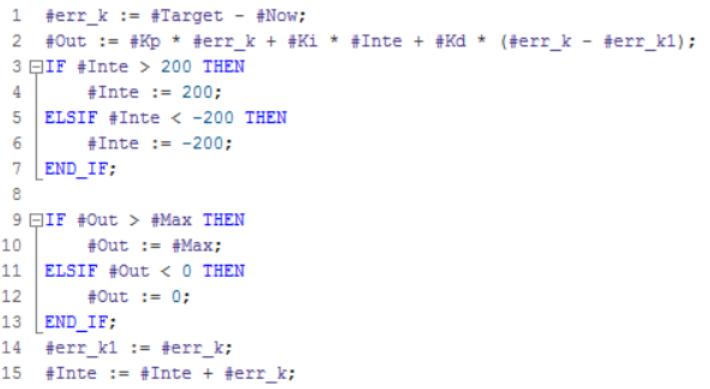
\includegraphics[width=.8\textwidth]{figure/单回路控制-自写程序-代码.png} 
    \caption{主水箱液位单回路控制手写代码} % caption是图片的标题
    % \label{img} % 此处的label相当于一个图片的专属标志,目的是方便上下文的引用
\end{figure}
\begin{figure}[H]
    \centering % 居中 
    % 图片文件的相对路径
    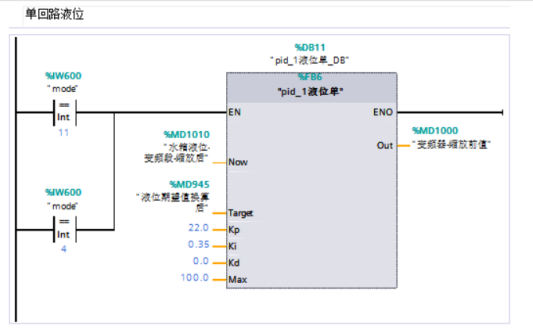
\includegraphics[width=.8\textwidth]{figure/单回路控制-自写程序-调用程序图.png} 
    \caption{主水箱液位单回路控制手写程序的调用程序图} % caption是图片的标题
    % \label{img} % 此处的label相当于一个图片的专属标志,目的是方便上下文的引用
\end{figure}

经参数整定后,PID控制器的各参数如下:
\begin{table}[H] % 防止表格乱跑
\centering % 居中
\begin{tabular}{cc} % 指明列数
    \toprule % 顶部粗线
    参数 & 整定值 \\
    \midrule % 中间细线
    Kp & 22.0 \\
    Ki & 0.35 \\
    Kd & 0.0 \\
    \bottomrule % 底部粗线
\end{tabular}
\caption{PID控制器参数整定结果} % 标题
\end{table}

%%%
\subsubsection{运行结果}
基于自行设计的PID控制器的主水箱液位单回路控制系统的控制效果如下:
\begin{figure}[H]
    \centering % 居中 
    % 图片文件的相对路径
    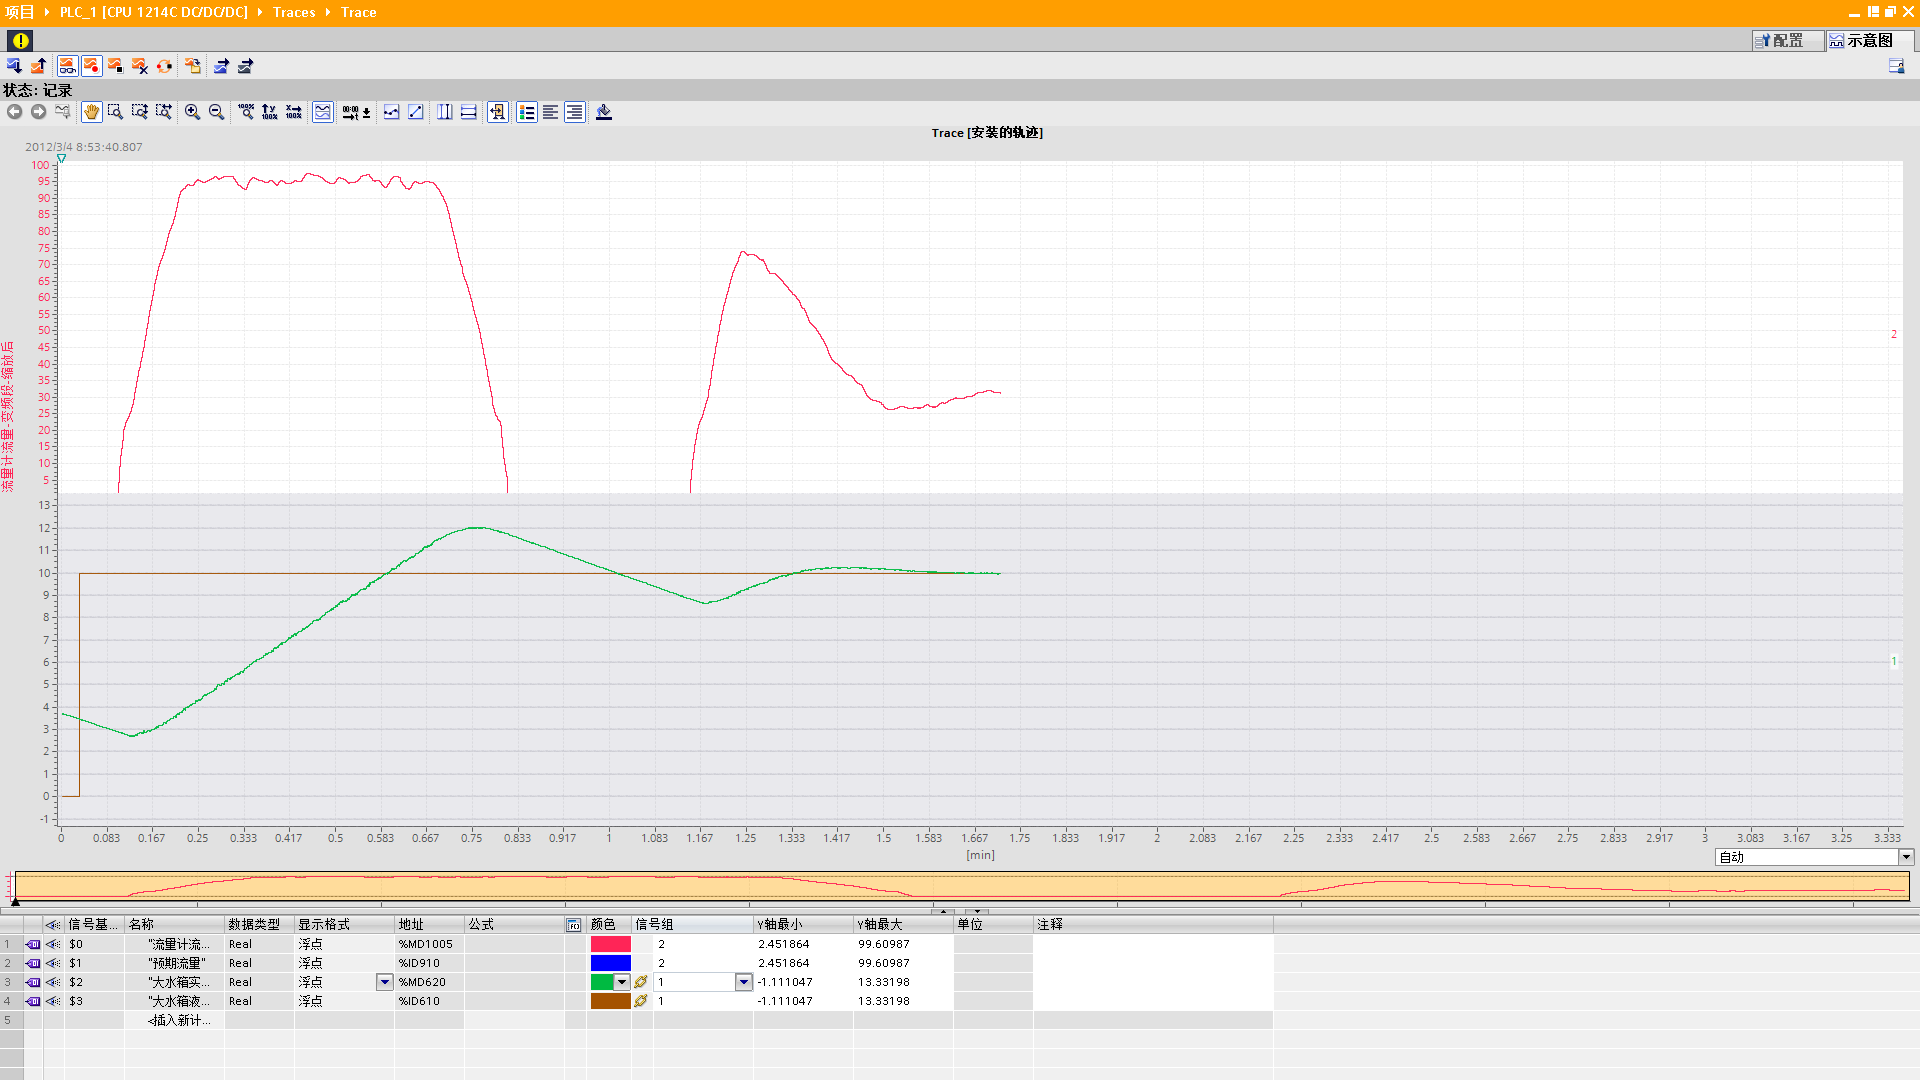
\includegraphics[width=1\textwidth]{figure/单回路控制效果.png} 
    \caption{主水箱液位单回路控制手写程序的控制效果} % caption是图片的标题
    % \label{img} % 此处的label相当于一个图片的专属标志,目的是方便上下文的引用
\end{figure}

对比使用PID模块的主水箱液位单回路控制系统,基于自行设计的PID控制器的控制效果要更好一些。

%%
\subsection{主水箱液位-流量串级控制系统设计(基于PID模块)}
%%%
\subsubsection{控制系统设计}
针对串级控制系统设计,我们仍选择主水箱作为主要被控对象,主水箱液位为主被控量,将主水箱对应的变频段管道作为副被控对象,其水流流量为副被控量,主副控制器均使用PID控制器,此外执行器和检测变送器与单回路控制系统均保持一致。系统整体构成一个双闭环的主水箱液位-流量串级控制系统,外环对主水箱液位进行控制,其输出为期望的水管流量,输入到内环;内环根据外环的给定值,对供水的变频段管道流量进行快速调节。主水箱液位-流量串级控制系统框图如下所示:
\begin{figure}[H]
    \centering % 居中 
    % 图片文件的相对路径
    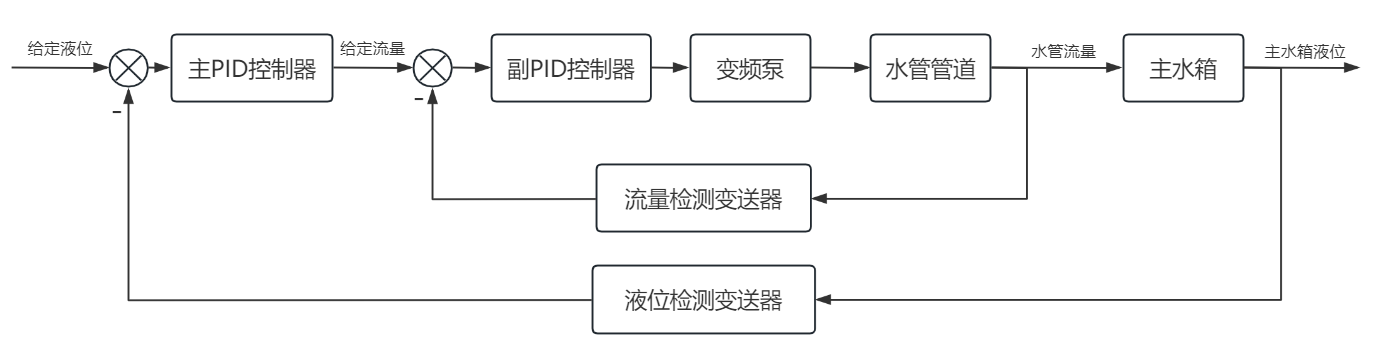
\includegraphics[width=1\textwidth]{figure/主水箱液位-流量串级控制系统框图.png} 
    \caption{主水箱液位-流量串级控制系统框图} % caption是图片的标题
    % \label{img} % 此处的label相当于一个图片的专属标志,目的是方便上下文的引用
\end{figure}

%%%
\subsubsection{程序设计}
此处采用PLC库中的PID模块构建串级控制系统中的主、副PID控制器部分,其程序设计图如下:
\begin{figure}[H]
    \centering % 居中 
    % 图片文件的相对路径
    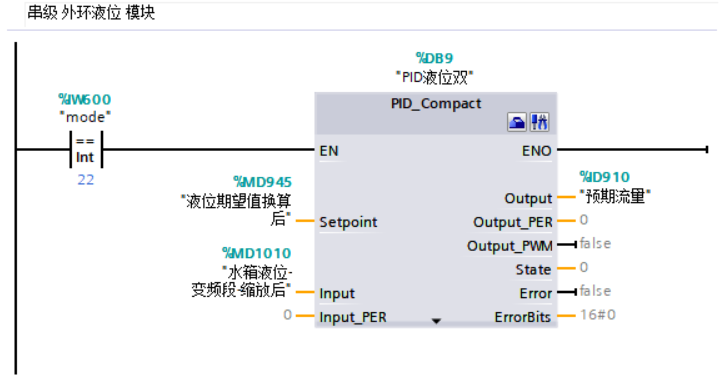
\includegraphics[width=.8\textwidth]{figure/串级-外环液位-模块.PNG} 
    \caption{外环液位控制程序图} % caption是图片的标题
    % \label{img} % 此处的label相当于一个图片的专属标志,目的是方便上下文的引用
\end{figure}
\begin{figure}[H]
    \centering % 居中 
    % 图片文件的相对路径
    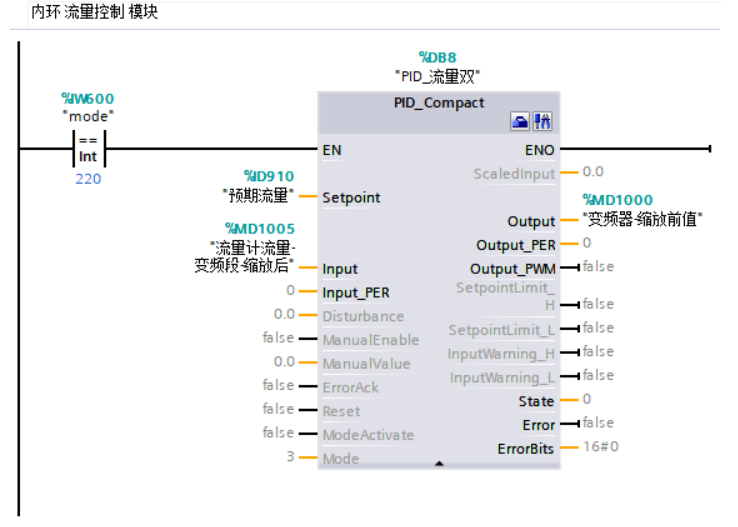
\includegraphics[width=.8\textwidth]{figure/串级-内环流量-模块.PNG} 
    \caption{内环流量控制程序图} % caption是图片的标题
    % \label{img} % 此处的label相当于一个图片的专属标志,目的是方便上下文的引用
\end{figure}

经参数整定后,最终使用的外环、内环对应的主、副PID控制器的各参数如下:
\begin{figure}[H]
    \centering % 居中 
    % 图片文件的相对路径
    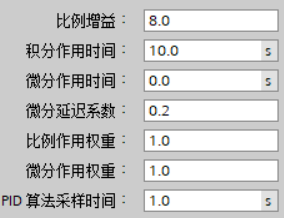
\includegraphics[width=.4\textwidth]{figure/串级-外环液位-模块-PID参数.PNG} 
    \caption{外环PID参数} % caption是图片的标题
    % \label{img} % 此处的label相当于一个图片的专属标志,目的是方便上下文的引用
\end{figure}
\begin{figure}[H]
    \centering % 居中 
    % 图片文件的相对路径
    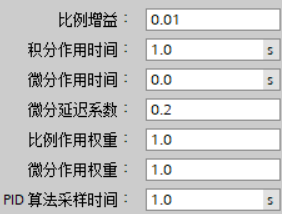
\includegraphics[width=.4\textwidth]{figure/串级-内环流量-模块-PID参数.PNG} 
    \caption{内环PID参数} % caption是图片的标题
    % \label{img} % 此处的label相当于一个图片的专属标志,目的是方便上下文的引用
\end{figure}

%%%
\subsubsection{控制效果展示}
主水箱液位-流量串级控制系统的控制效果展示如下:
\begin{figure}[H]
    \centering % 居中 
    % 图片文件的相对路径
    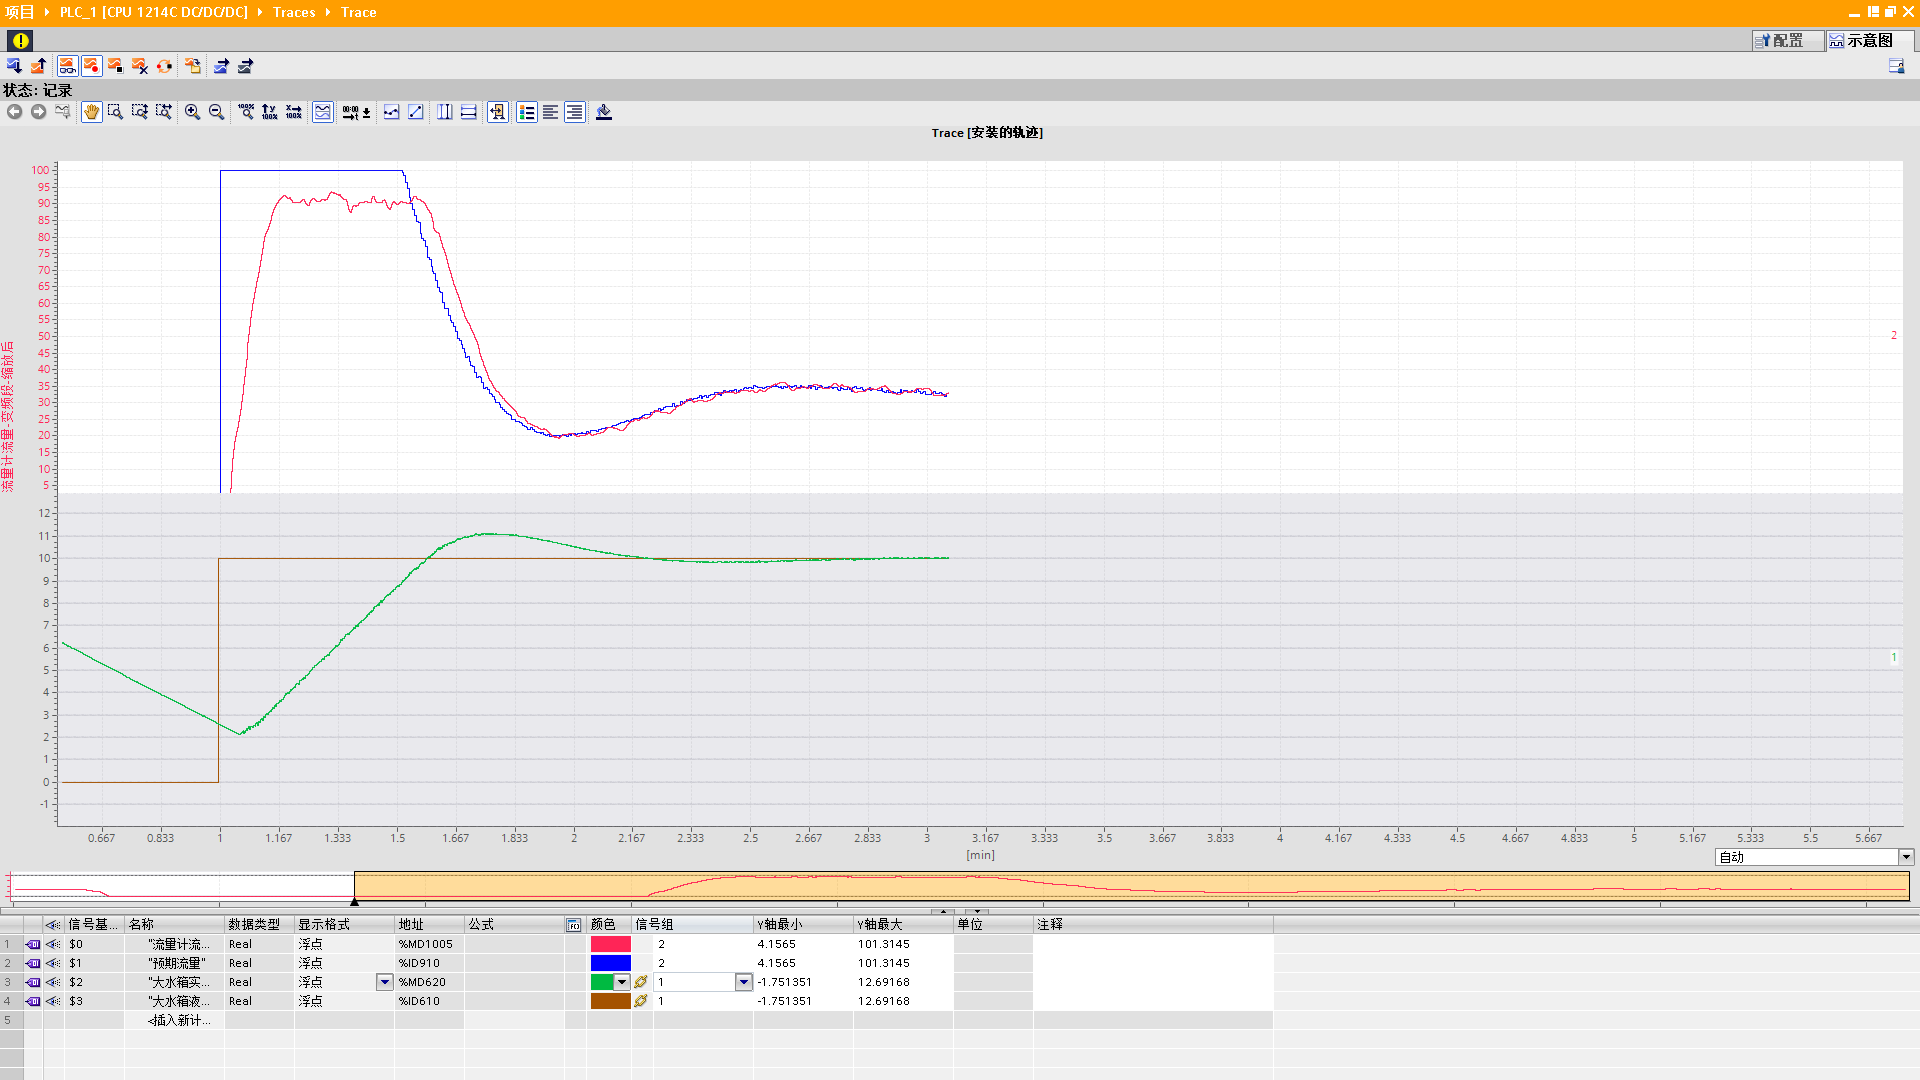
\includegraphics[width=1\textwidth]{figure/串级控制效果.png} 
    \caption{主水箱液位-流量串级控制系统效果} % caption是图片的标题
    % \label{img} % 此处的label相当于一个图片的专属标志,目的是方便上下文的引用
\end{figure}
可以看到,副回路所控制的管道流量基本上可以做到实时跟踪给定值,因此主水箱液位也能够以较好的方式稳定在给定值上,总体上该串级系统整体上的控制效果是比较好的。

%%
\subsection{主水箱液位-流量串级控制系统设计(基于自行设计的PID)}
%%%
\subsubsection{控制系统设计}
在我们自定义的双回路PID控制系统中,我们采用了一种精细的控制策略:内环负责控制流量,而外环负责控制液位。这种双回路结构使得控制更加精确和灵活,因为它允许我们分别对流量和液位进行独立调节,从而更有效地达到控制目标。

在内环,我们选择了增量式PID控制。这种控制方法非常适合处理流量控制的需求,因为它能够有效地应对系统的快速变化和噪声干扰,防止过度调整。增量式PID通过计算控制量的增量,提供了对流量变化的快速且精确响应,同时减少了控制器的积分饱和风险,这对于保持流量的稳定运行至关重要。

对于外环,我们选择了位置式PID控制。位置式PID控制适用于液位控制,因为它提供了对长期稳态误差的有效补偿。这种控制方式有助于确保液位保持在设定的目标值,即使在外部条件发生变化时也能保持相对稳定。由于液位控制通常不需要频繁和快速的调整,位置式PID的这种特性使其成为控制液位的理想选择。

在串级控制系统中,为了确保控制的有效性和协调性,我们特别设置了内环控制频率是外环控制频率的10倍,这种差异化的频率设置不仅增强了系统的灵活性和反应速度,还保障了整个控制过程的稳定性和准确性。因此,我们的双回路PID控制系统得以在各种运行条件下展现卓越的性能。

%%%
\subsubsection{程序设计}
在使用博图软件进行控制系统设计时,我们首先创建了两个循环中断的组织块(OB),以适应两个控制回路的不同时间需求。其中一个组织块设定了300毫秒的循环时间,用于较慢的外回路控制;而另一个则设定了30毫秒的循环时间,用于快速响应的内回路控制。这样的设置能够确保每个回路按照其需求运行,从而实现高效的控制。

在我们的控制系统设计中,对于内回路的流量控制,为了使内回路对外回路控制的快速跟随。我们选择了提升控制速度。这种方法确保了流量控制能够迅速响应外回路液位控制的变化,从而保持整个系统的协调运行。在外回路的液位控制中,我们采用了PI控制器,这主要是为了减少稳态误差。在液位控制应用中,这种策略意味着即使面对外部条件的变化或系统的扰动,PI控制器也能有效地确保液位稳定在设定值。此外,比例控制部分的快速响应特性对提高系统的整体反应速度至关重要,特别是在液位发生变化时,快速调整能够显著提高系统的调节效率。
\begin{figure}[H]
    \centering % 居中 
    % 图片文件的相对路径
    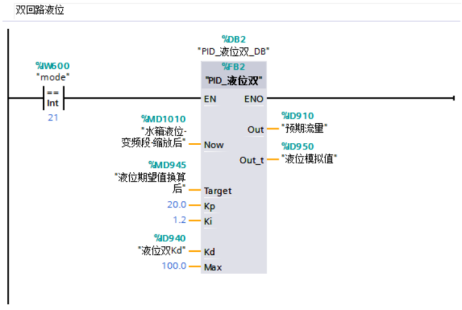
\includegraphics[width=.8\textwidth]{figure/串级-外环液位-手写-调用.PNG} 
    \caption{外环液位控制代码调用} % caption是图片的标题
    % \label{img} % 此处的label相当于一个图片的专属标志,目的是方便上下文的引用
\end{figure}
\begin{figure}[H]
    \centering % 居中 
    % 图片文件的相对路径
    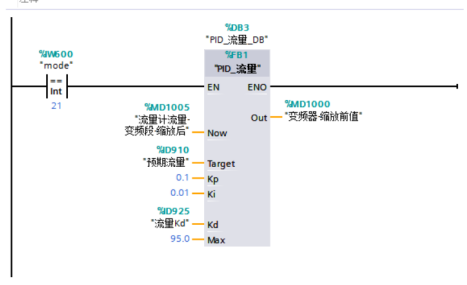
\includegraphics[width=0.8\textwidth]{figure/串级-内环流量-手写-调用.PNG} 
    \caption{内环流量控制代码调用} % caption是图片的标题
    % \label{img} % 此处的label相当于一个图片的专属标志,目的是方便上下文的引用
\end{figure}
\begin{figure}[H]
    \centering % 居中 
    % 图片文件的相对路径
    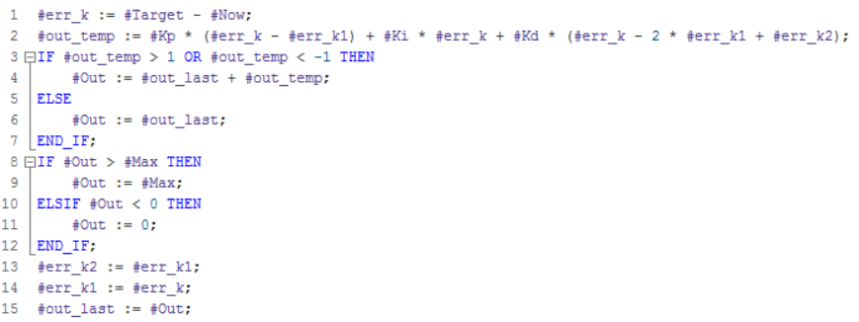
\includegraphics[width=1\textwidth]{figure/串级-内环流量-手写-代码.PNG} 
    \caption{内环流量控制代码} % caption是图片的标题
    % \label{img} % 此处的label相当于一个图片的专属标志,目的是方便上下文的引用
\end{figure}

外环、内环PID控制器参数的整定结果如下所示:
\begin{table}[H] % 防止表格乱跑
\centering % 居中
\begin{tabular}{cc} % 指明列数
    \toprule % 顶部粗线
    外环PID参数 & 内环PID参数 \\
    \midrule % 中间细线
    Kp = 20.0 &  Kp = 0.1\\
    Ki = 1.2 & Ki = 0.01 \\
    Kd = 0.0 & Kd = 0.0 \\
    \bottomrule % 底部粗线
\end{tabular}
\caption{串级控制系统PID控制器参数整定结果} % 标题
\end{table}

%%%
\subsubsection{运行结果}
基于自行设计的PID控制器的串级控制系统的控制效果如下图所示:
\begin{figure}[H]
    \centering % 居中 
    % 图片文件的相对路径
    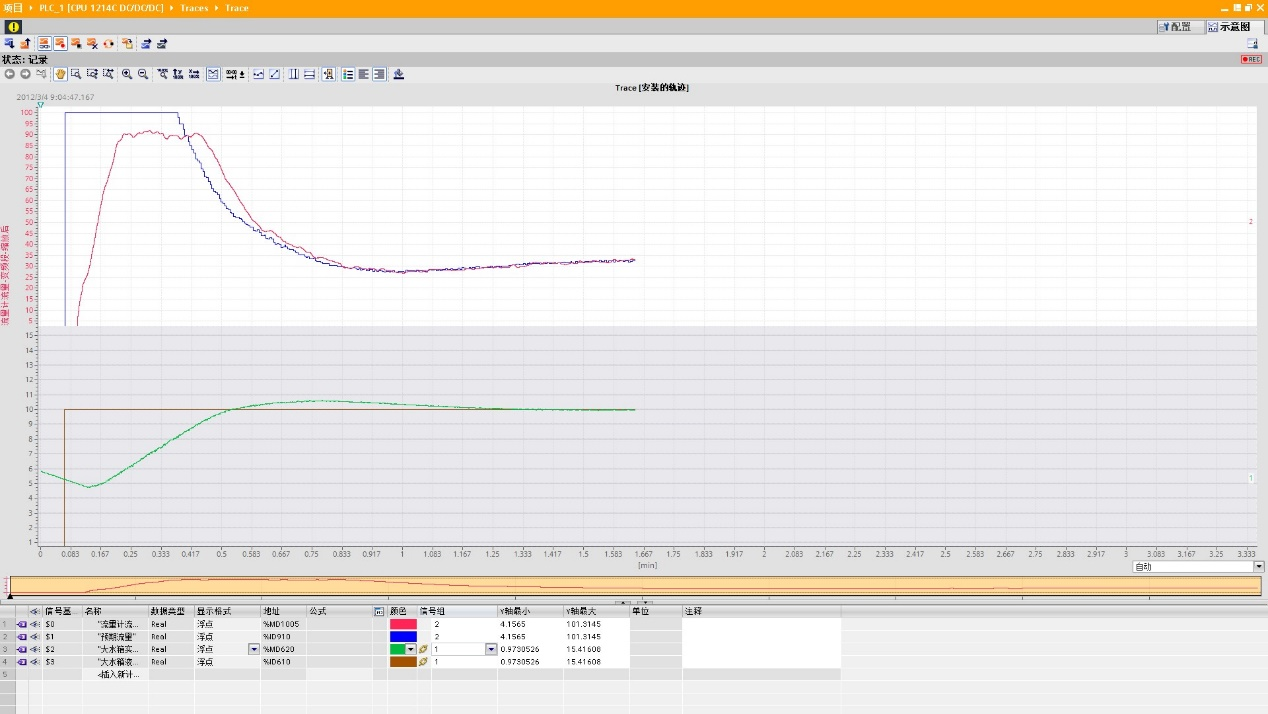
\includegraphics[width=1\textwidth]{figure/串级控制-手写-控制效果.png} 
    \caption{基于自行设计的PID控制器的串级控制系统的控制效果} % caption是图片的标题
    % \label{img} % 此处的label相当于一个图片的专属标志,目的是方便上下文的引用
\end{figure}

%%
\subsection{主-副水箱液位双闭环比值控制系统设计}
%%%
\subsubsection{控制系统设计}
比值控制是一种相较单回路控制更加复杂的控制策略,被广泛应用于化工炼油等工业生产过程中。比值控制实际上是一种实现两个或两个以上参数符合一定比例关系的控制系统,一般以两种物料的比例作为被控量。比值控制策略具有很多种实现形式,如开环比值控制、单闭环比值控制、双闭环比值控制,以及变比值控制等。

在本次实习中,我们设计了一个针对主副水箱液位的双闭环比值控制系统,以控制主、副水箱液位之间的比例关系。在该系统中,主、副水箱作为被控对象,其液位为被控量,两水箱的液位计用来实现液位的检测变送;变频泵和电磁阀则分别作为两个控制回路的执行器。在双闭环比值控制系统中,两个控制回路之间相对独立,故主、副水箱之间不存在耦合关系。此外,我们选择副水箱液位作为比值控制系统中的主动量,主水箱液位作为从动量,将副水箱液位的实际测量值经比例运算后作为主水箱液位的给定值。主-副水箱液位双闭环比值控制系统框图如下图所示:
\begin{figure}[H]
    \centering % 居中 
    % 图片文件的相对路径
    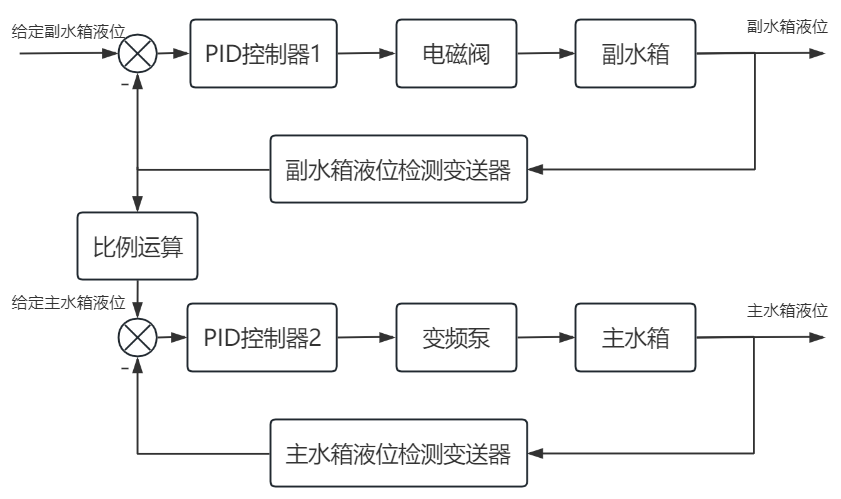
\includegraphics[width=.8\textwidth]{figure/比值控制系统框图.png} 
    \caption{主-副水箱液位双闭环比值控制系统框图} % caption是图片的标题
    % \label{img} % 此处的label相当于一个图片的专属标志,目的是方便上下文的引用
\end{figure}

%%%
\subsubsection{程序设计}
双闭环比值控制系统的程序主要包含两个单回路闭环控制部分,以及从副水箱实际液位经比例运算后得到主水箱液位控制给定值的程序段:
\begin{figure}[H]
    \centering % 居中 
    % 图片文件的相对路径
    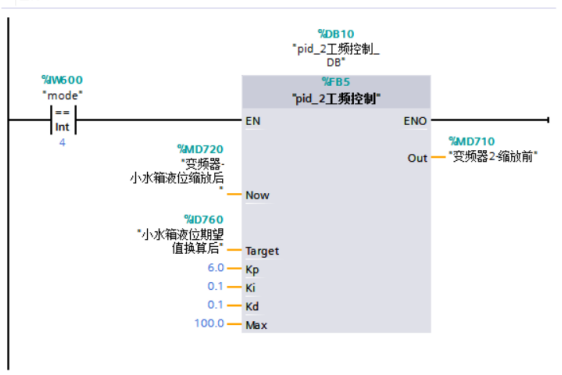
\includegraphics[width=.8\textwidth]{figure/比值控制-程序1.png} 
    \caption{副水箱液位单回路控制程序} % caption是图片的标题
    % \label{img} % 此处的label相当于一个图片的专属标志,目的是方便上下文的引用
\end{figure}
\begin{figure}[H]
    \centering % 居中 
    % 图片文件的相对路径
    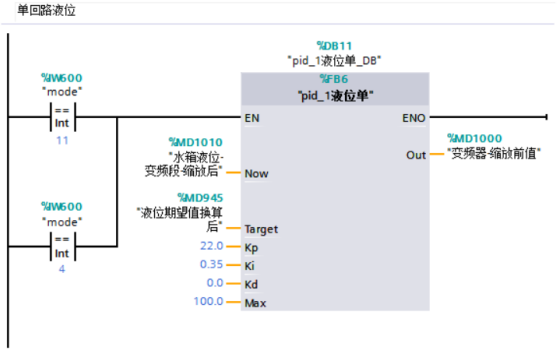
\includegraphics[width=.8\textwidth]{figure/比值控制-程序2.png} 
    \caption{主水箱液位单回路控制程序} % caption是图片的标题
    % \label{img} % 此处的label相当于一个图片的专属标志,目的是方便上下文的引用
\end{figure}
\begin{figure}[H]
    \centering % 居中 
    % 图片文件的相对路径
    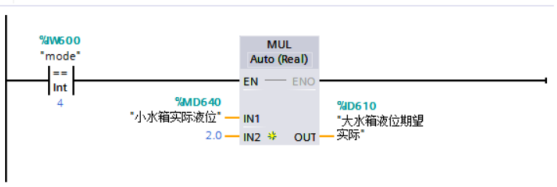
\includegraphics[width=.8\textwidth]{figure/比值控制-程序3.png} 
    \caption{比例运算部分的程序} % caption是图片的标题
    % \label{img} % 此处的label相当于一个图片的专属标志,目的是方便上下文的引用
\end{figure}

经参数整定后,双闭环比值控制系统的主、副水箱液位控制单回路的PID控制器参数分别如下所示:
\begin{table}[H] % 防止表格乱跑
\centering % 居中
\begin{tabular}{cc} % 指明列数
	\toprule % 顶部粗线
	主水箱液位控制回路 & 副水箱液位控制回路 \\
	\midrule % 中间细线
	Kp = 22.0 &  Kp = 6.0\\
	Ki = 0.35 & Ki = 0.1 \\
	Kd = 0.0 & Kd = 0.1 \\
	\bottomrule % 底部粗线
\end{tabular}
\caption{比值控制系统PID控制器参数} % 标题
\end{table}

%%%
\subsubsection{控制效果展示}
主-副水箱液位双闭环比值控制系统的控制效果如下图所示:
\begin{figure}[H]
    \centering % 居中 
    % 图片文件的相对路径
    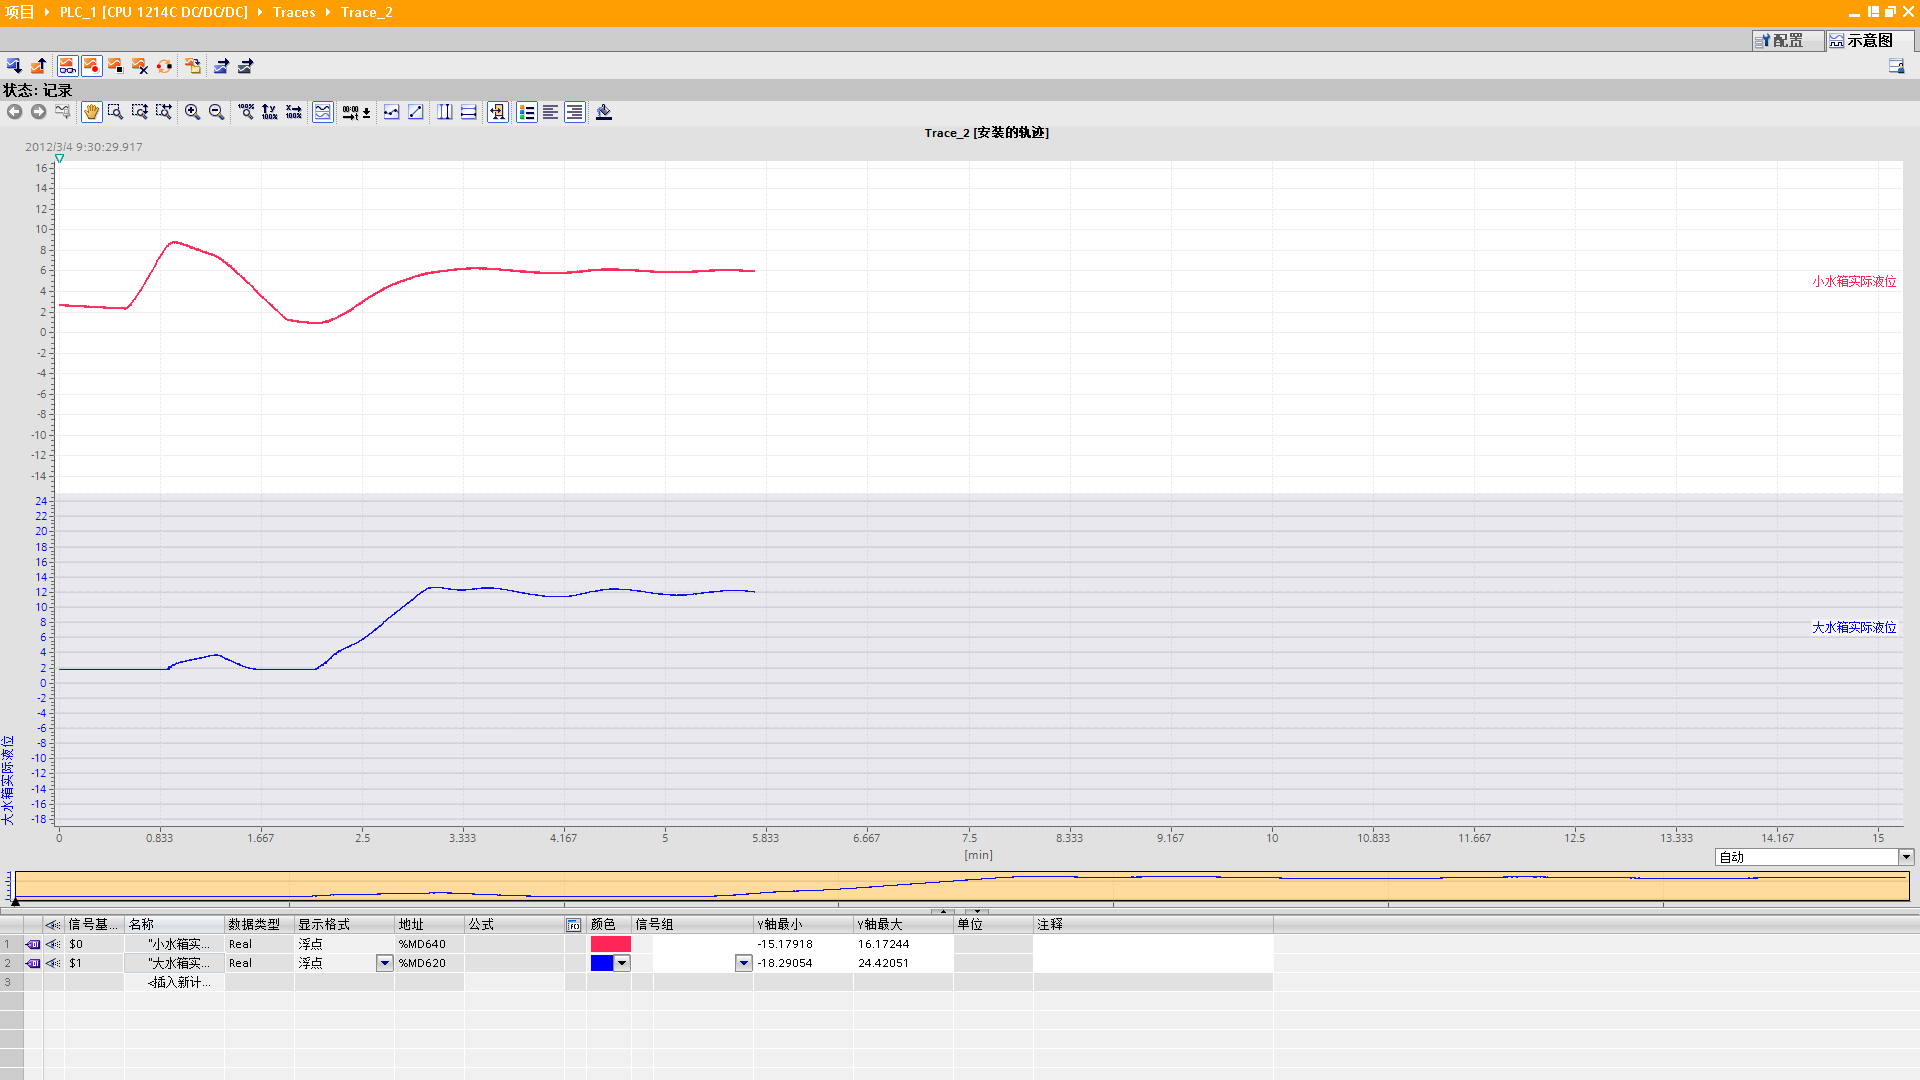
\includegraphics[width=1\textwidth]{figure/比值控制效果1.png} 
    \caption{比值控制效果图1} % caption是图片的标题
    % \label{img} % 此处的label相当于一个图片的专属标志,目的是方便上下文的引用
\end{figure}
\begin{figure}[H]
    \centering % 居中 
    % 图片文件的相对路径
    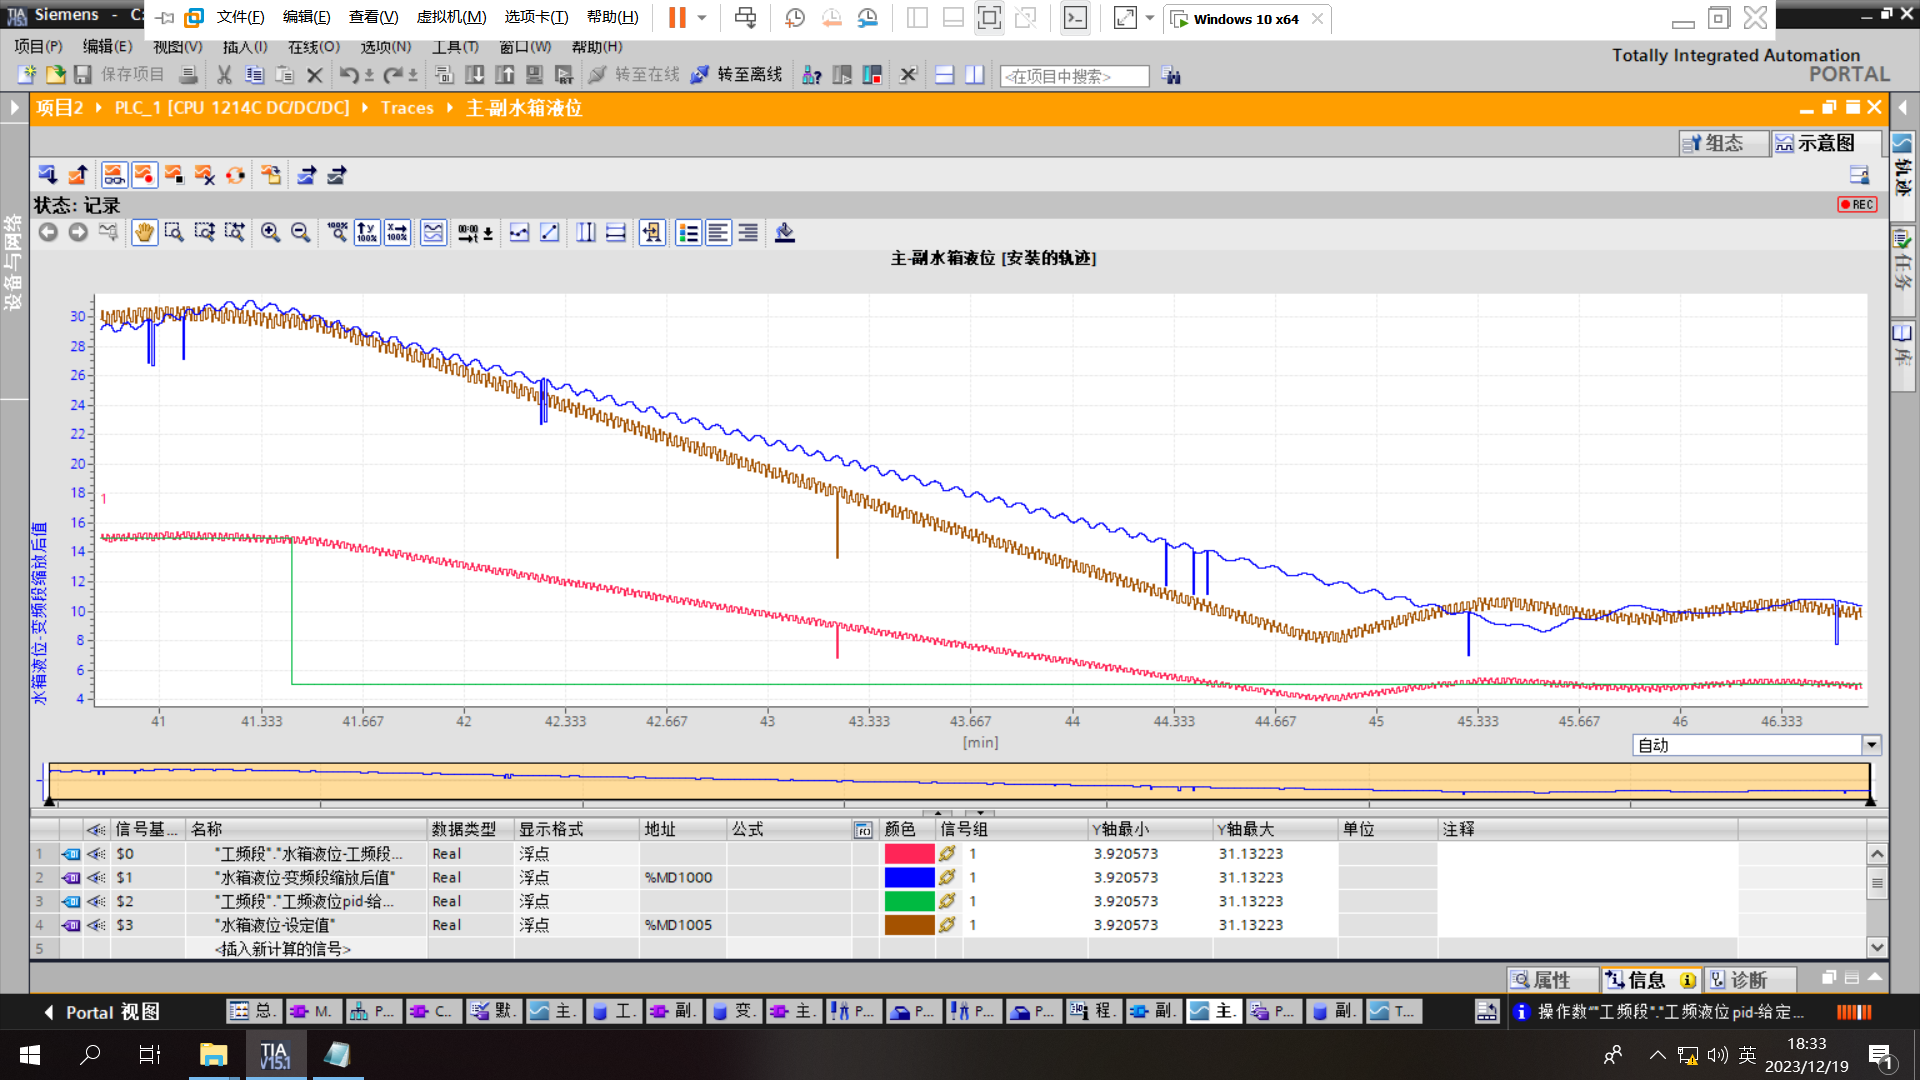
\includegraphics[width=1\textwidth]{figure/比值控制效果2.png} 
    \caption{比值控制效果图2} % caption是图片的标题
    % \label{img} % 此处的label相当于一个图片的专属标志,目的是方便上下文的引用
\end{figure}
可以看到,在调节过程中,主水箱液位基本可以按照给定的比例(2:1)跟随副水箱液位的变化,实现了比较好的控制效果。

%%
\subsection{双容水箱液位串级控制系统设计}
%%%
\subsubsection{控制系统设计}
我们使用实验台提供的主、副两个水箱构成双容水箱,并将其作为被控对象,设计了一个双容水箱液位串级控制系统。由于主、副水箱之间已经有管道连接,只需将该管道的手动阀打开即可在主、副两水箱之间建立耦合关系。

双容水箱液位串级控制系统的大致思路为:通过控制副水箱的液位以间接控制主水箱的供水流量,从而达到控制主水箱液位的目的。其中,通过设置相应手动阀的开关可以将变频泵的供水引至副水箱中,使得可以通过变频泵调节副水箱液位。在该控制系统中,外环以主水箱液位为主被控量,由主水箱液位变送器进行检测;内环以副水箱液位为副被控量,可通过副水箱液位变送器检测;外环的输出为期望的副水箱液位,实际上与主、副水箱之间水管的流量成正相关关系,外环输出给到内环进行调节,使得副水箱液位可以满足对于流量的需求。双容水箱液位串级控制系统框图如下所示:
\begin{figure}[H]
    \centering % 居中 
    % 图片文件的相对路径
    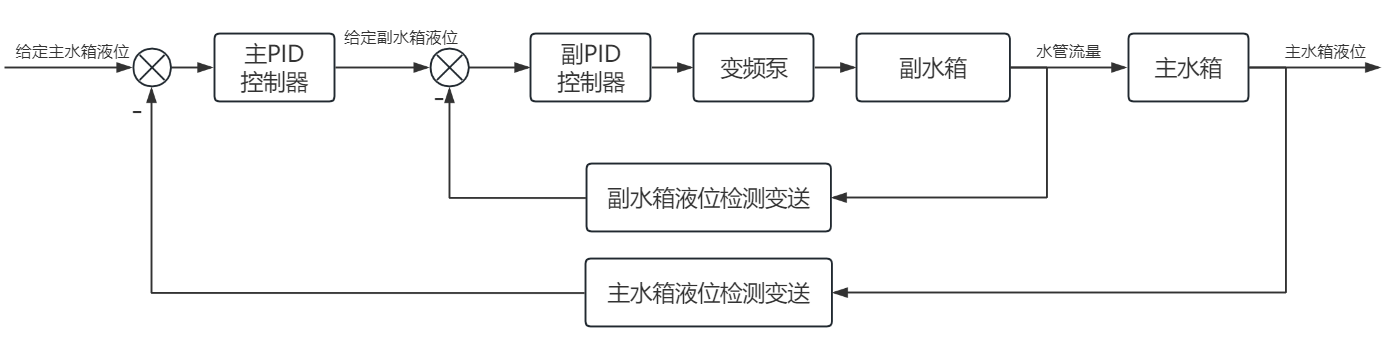
\includegraphics[width=1\textwidth]{figure/双容水箱控制系统框图.png} 
    \caption{双容水箱液位串级控制系统框图} % caption是图片的标题
    % \label{img} % 此处的label相当于一个图片的专属标志,目的是方便上下文的引用
\end{figure}

%%%
\subsubsection{程序设计}
双容水箱液位串级控制系统主要的程序设计主要包含一个针对主水箱液位的外环控制回路以及一个针对副水箱液位的内环控制回路,具体的程序设计图如下所示:
\begin{figure}[H]
    \centering % 居中 
    % 图片文件的相对路径
    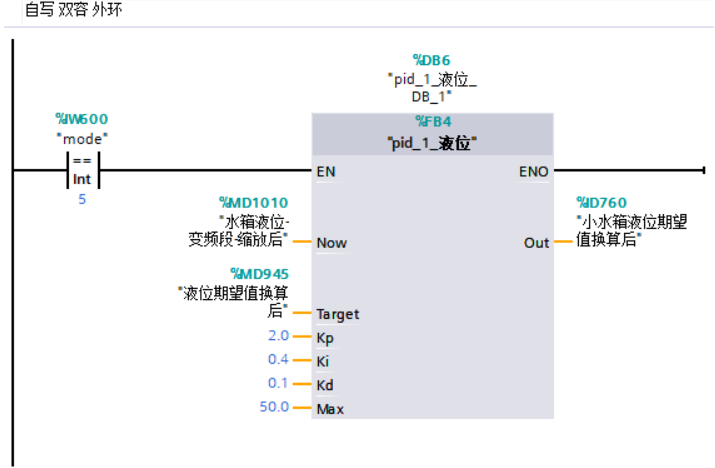
\includegraphics[width=0.8\textwidth]{figure/双容-外环-自写.png} 
    \caption{双容水箱液位串级控制系统-外环程序} % caption是图片的标题
    % \label{img} % 此处的label相当于一个图片的专属标志,目的是方便上下文的引用
\end{figure}
\begin{figure}[H]
    \centering % 居中 
    % 图片文件的相对路径
    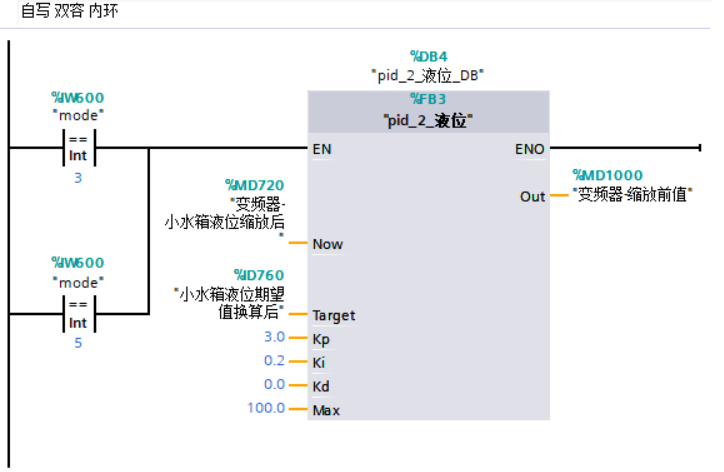
\includegraphics[width=0.8\textwidth]{figure/双容-内环-自写.png} 
    \caption{双容水箱液位串级控制系统-内环程序} % caption是图片的标题
    % \label{img} % 此处的label相当于一个图片的专属标志,目的是方便上下文的引用
\end{figure}

经参数整定后,双容水箱串级控制系统的主、副控制回路的PID控制器参数分别如下所示:
\begin{table}[H] % 防止表格乱跑
\centering % 居中
\begin{tabular}{cc} % 指明列数
	\toprule % 顶部粗线
	水箱液主控制回路 & 流量副控制回路 \\
	\midrule % 中间细线
	Kp = 22.0 &  Kp = 6.0\\
	Ki = 0.35 & Ki = 0.1 \\
	Kd = 0.0 & Kd = 0.1 \\
	\bottomrule % 底部粗线
\end{tabular}
\caption{双容水箱串级控制系统PID控制器参数} % 标题
\end{table}

%%%
\subsubsection{控制效果展示}
我们设计的双容水箱液位串级控制系统的控制效果如下图所示:
\begin{figure}[H]
    \centering % 居中 
    % 图片文件的相对路径
    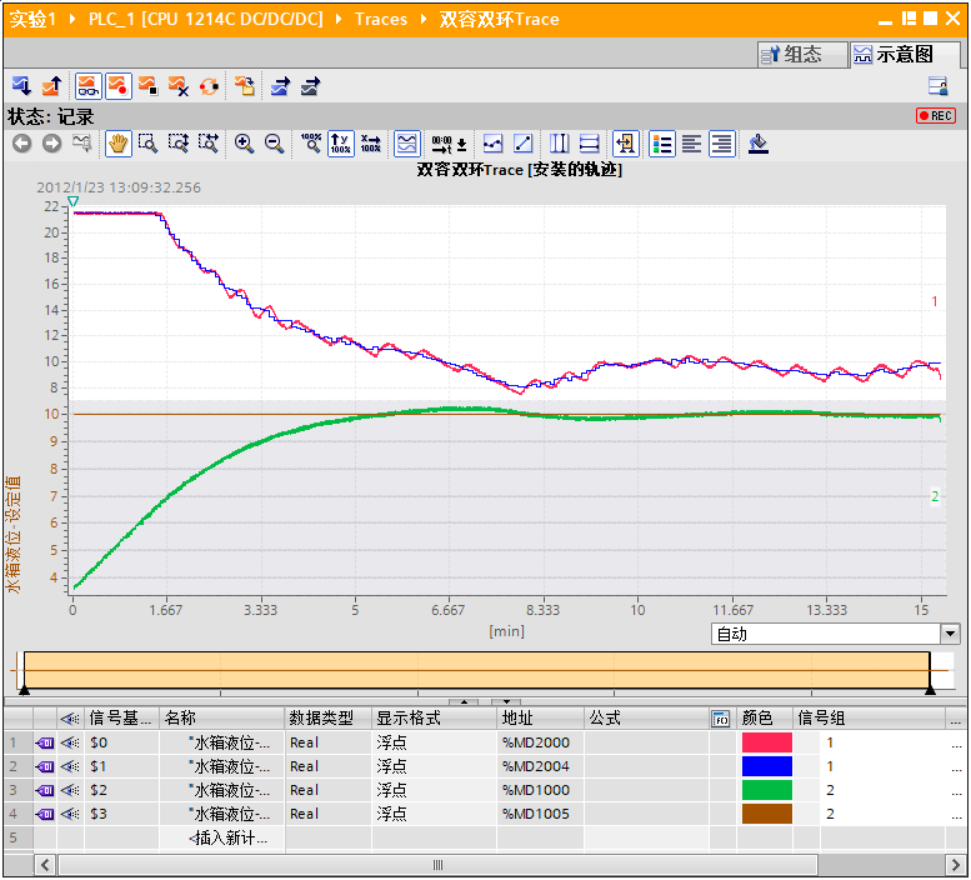
\includegraphics[width=0.8\textwidth]{figure/双容水箱控制效果图.png} 
    \caption{双容水箱液位串级控制系统控制效果} % caption是图片的标题
    % \label{img} % 此处的label相当于一个图片的专属标志,目的是方便上下文的引用
\end{figure}
从上图可以看出,内环所控制的副水箱液位基本可以做到对给定值的跟随。由于主、副水箱之间的水管管径比较小,且副水箱的水箱高度较低,因此该处的水流流量存在比较明显的限制。当给定的副水箱液位值下降过快时,副水箱放水的流量可能无法很好的满足其要求,这是我们在进行双容水箱控制系统设计时发现的一个比较棘手的问题。

%%
\subsection{针对流量干扰的前馈-反馈控制系统设计}
%%%
\subsubsection{控制系统设计}
在前馈-反馈控制系统的设计中,我们首先选择以副水箱作为被控对象,以副水箱液位作为被控量,构建一个基于反馈控制的单回路闭环控制结构。然后针对该系统中供水管道流量参数可能出现的干扰设计一个前馈控制器,进而得到一个针对副水箱液位控制和抑制流量干扰的前馈-反馈控制系统。在该系统的实现中,我们通过实验得到了基于流量变化对副水箱液位影响进行抵消的补偿函数,进而得到了该补偿函数对应的前馈控制器的作用方式。

如果流量的变化足够大以至于影响到液位,系统会启动前馈控制器进行进一步的调整。这一步骤是为了确保即使在较大的流量变化下,液位也能够被有效地控制,并最终达到一个平衡状态。通过这种前馈和反馈的结合,控制系统能够在各种条件下有效地维持水箱液位的稳定,从而优化整个系统的控制性能。前馈-反馈控制系统框图如下所示:
\begin{figure}[H]
    \centering % 居中 
    % 图片文件的相对路径
    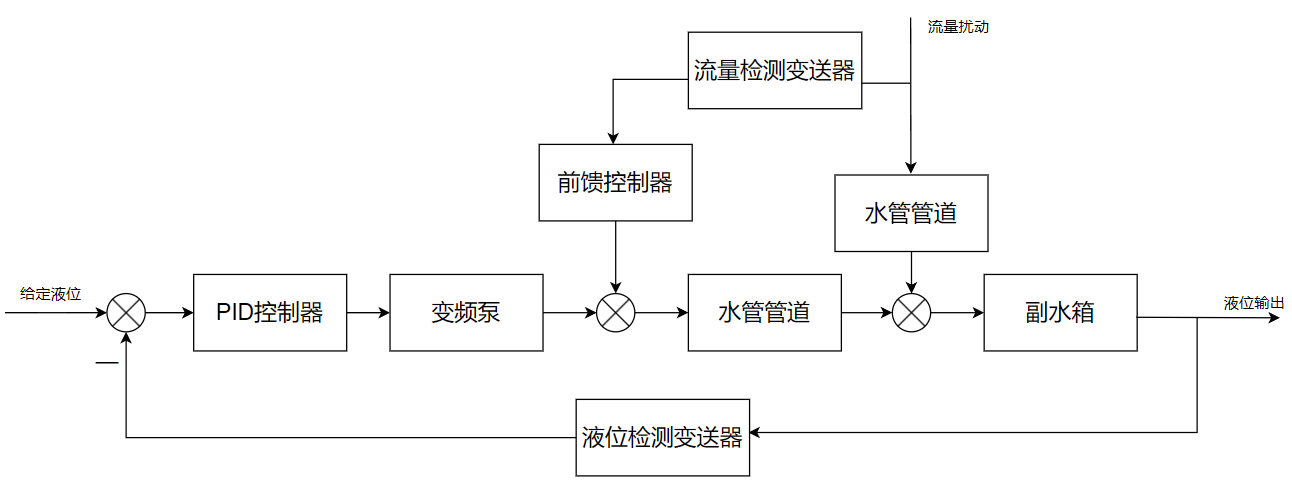
\includegraphics[width=0.8\textwidth]{figure/前馈反馈控制系统框图.png} 
    \caption{前馈反馈控制系统框图} % caption是图片的标题
    % \label{img} % 此处的label相当于一个图片的专属标志,目的是方便上下文的引用
\end{figure}

%%%
\subsubsection{程序设计}
前馈-反馈控制系统的程序图以及对应代码如下所示:
\begin{figure}[H]
    \centering % 居中 
    % 图片文件的相对路径
    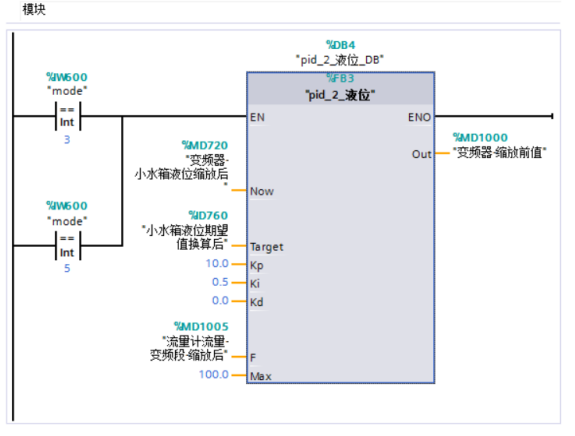
\includegraphics[width=0.8\textwidth]{figure/前馈反馈-程序1.png} 
    \caption{前馈反馈控制系统程序调用图} % caption是图片的标题
    % \label{img} % 此处的label相当于一个图片的专属标志,目的是方便上下文的引用
\end{figure}
\begin{figure}[H]
    \centering % 居中 
    % 图片文件的相对路径
    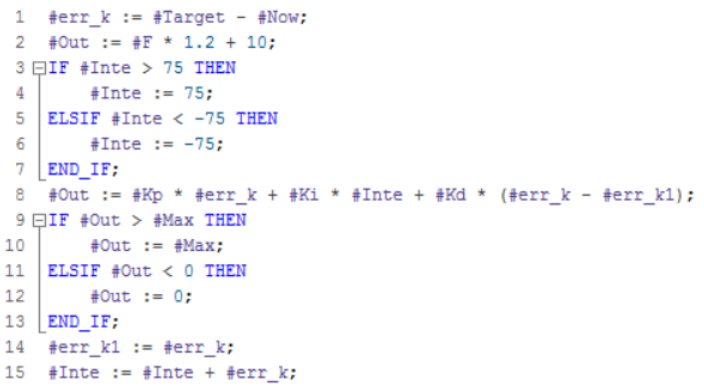
\includegraphics[width=0.8\textwidth]{figure/前馈反馈-程序2.png} 
    \caption{前馈反馈控制系统代码实现} % caption是图片的标题
    % \label{img} % 此处的label相当于一个图片的专属标志,目的是方便上下文的引用
\end{figure}

经参数整定后,前馈-反馈控制系统中的单回路PID控制器参数如下所示:
\begin{table}[H] % 防止表格乱跑
\centering % 居中
\begin{tabular}{cc} % 指明列数
	\toprule % 顶部粗线
	PID参数 & 整定值 \\
	\midrule % 中间细线
	Kp &  10.0 \\
	Ki & 0.5 \\
	Kd & 0.0 \\
	\bottomrule % 底部粗线
\end{tabular}
\caption{前馈-反馈控制系统单回路PID控制器参数} % 标题
\end{table}

%%%
\subsubsection{控制效果展示}
前馈-反馈控制系统对副水箱液位的调节效果如下图所示:
\begin{figure}[H]
    \centering % 居中 
    % 图片文件的相对路径
    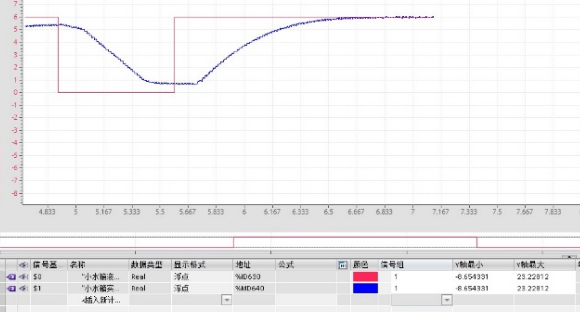
\includegraphics[width=0.8\textwidth]{figure/前馈反馈-控制效果.png} 
    \caption{前馈反馈控制系统控制效果展示} % caption是图片的标题
    % \label{img} % 此处的label相当于一个图片的专属标志,目的是方便上下文的引用
\end{figure}

%
\section{HMI交互界面设计}
本次实习选择台达B10E615 HMI显示面板作为本次实习的人机交换界面。HMI通过以太网与PLC建立有线网络通讯。界面设计通过台达公司的DOPSoft开发软件为水箱液位控制系统设计交互界面。本次界面设计较好的满足了实际生产过程中的需求。通过登录界面,控制人员对于系统的访问与控制。并且对于不同用户的登录,做出了控制权限的区分与管理。综上所述,该人机交互界面,完美的完成了实际生产需求。接下来进行详细的开发与技术细节介绍。

%%
\subsection{创建新项目}
本次实习所使用的台达HMI显示面板需要使用上位机开发软件DOPSoft。实习所给的软件中已经给出无需重现下载。打开软件后,出现如图\ref{fig:img1}的设计主界面,单击File—New创建新项目。
\begin{figure}[H]
    \centering % 居中 
    % 图片文件的相对路径
    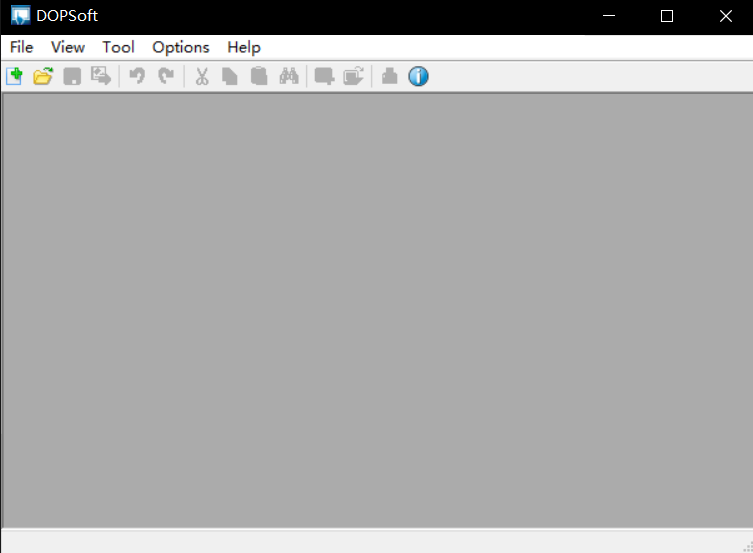
\includegraphics[width=0.8\textwidth]{figure/设计主界面.png} 
    \caption{设计主界面} % caption是图片的标题
    \label{fig:img1} % 此处的label相当于一个图片的专属标志,目的是方便上下文的引用
\end{figure}

如图\ref{fig:img2}选择本次实验所使用的B10E615触摸屏。单击下一步进入通信界面选项。完成型号选择后,弹出HMI通讯设置界面如图\ref{fig:img3}所示。
\begin{figure}[H]
    \centering % 居中 
    % 图片文件的相对路径
    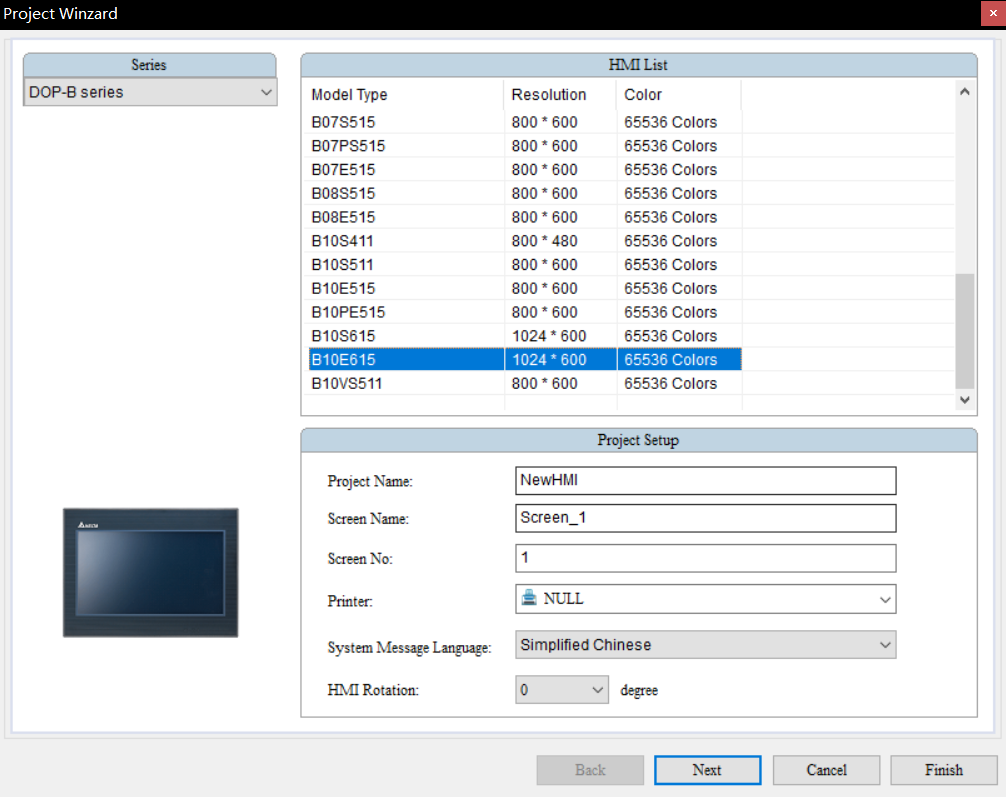
\includegraphics[width=0.8\textwidth]{figure/HMI型号选取界面.png} 
    \caption{HMI型号选取界面} % caption是图片的标题
    \label{fig:img2} % 此处的label相当于一个图片的专属标志,目的是方便上下文的引用
\end{figure}

HMI显示屏可以通过COM口或以太网接口进行通讯。如图\ref{fig:img3}所示,该显示屏有三个COM口和一个Ethernet1口选项。本次实习使用以太网作为通信接口。因此取消勾选默认的COM2口后,勾选Ethernet1。
创建新网络设备,选择控制器为S7 1200(ISO TCP)并设置Controller IP为对应的PLC地址。这里我们设置为我们本次使用的PLC的地址 192.168.1.95。点击Finish后进入设计主界面。
\begin{figure}[H]
    \centering % 居中 
    % 图片文件的相对路径
    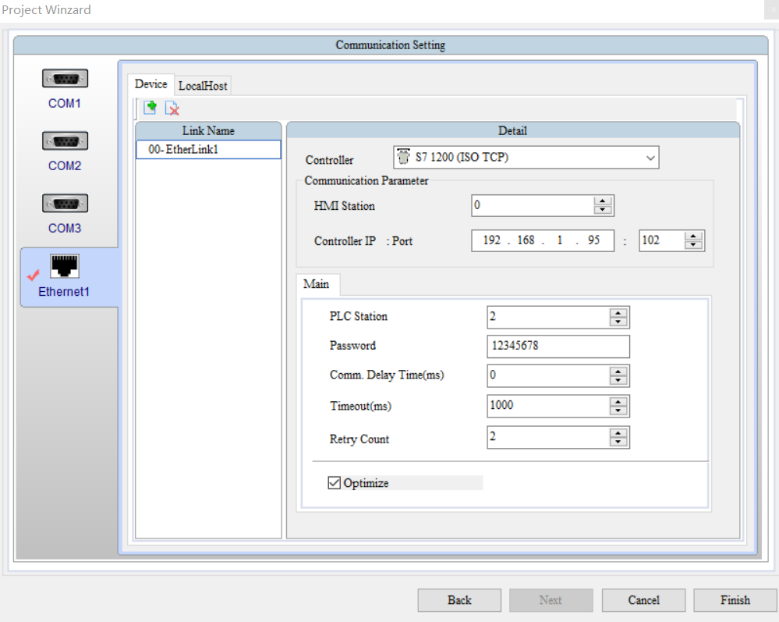
\includegraphics[width=0.8\textwidth]{figure/HMI通讯设置界面.png} 
    \caption{HMI通讯设置界面} % caption是图片的标题
    \label{fig:img3} % 此处的label相当于一个图片的专属标志,目的是方便上下文的引用
\end{figure}

%%
\subsection{主界面设计}
%%%
\subsubsection{登录界面设计}
登陆界面包括小组信息,系统名称,用户选择栏,密码输入栏和登录按钮。
\begin{figure}[H]
    \centering % 居中 
    % 图片文件的相对路径
    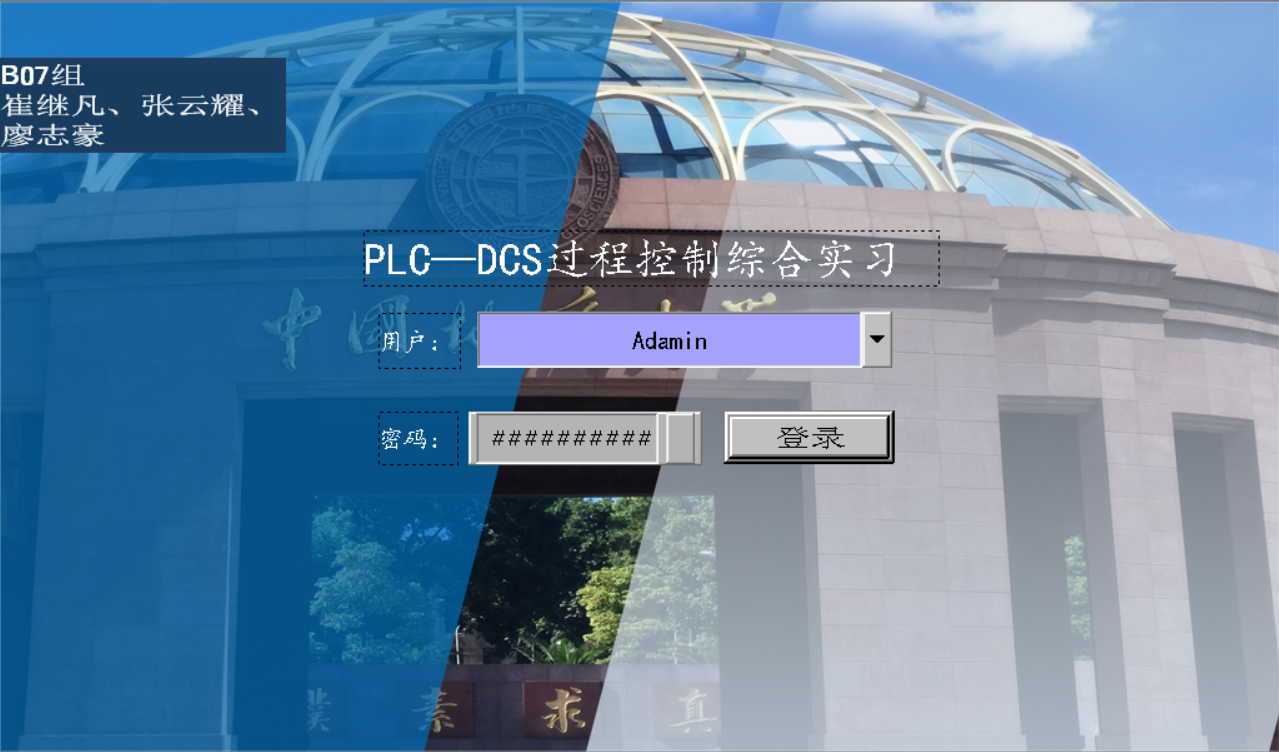
\includegraphics[width=0.8\textwidth]{figure/HMI登录界面仿真.png} 
    \caption{HMI登录界面仿真} % caption是图片的标题
    \label{fig:img4} % 此处的label相当于一个图片的专属标志,目的是方便上下文的引用
\end{figure}

本系统通过登录界面实现了管理者—操作员—访客的三级权限控制。例如,作为系统的管理者拥有最高级权限。登录后可以直接观察控制系统的全部状态信息,如某个底层传感器的数据。管理者有权调整系统所有控制器的参数以及状态。

二级权限:操作者可以通过图形化的界面观察到系统的系统的运行状态并及时的调整系统的运行参数与模式,但对于更底层的部分传感器数据与状态,无法观察与调整。但操作者的权限已经完全满足了系统调整所需的功能。

三级权限:访客,仅可以观察系统运行的状态,而无法调整系统运行的任何参数与状态,保证了系统的安全可靠。

登录界面会检查登录用户所输入密码与HMI内部存储器中存储的密码是否匹配。当不匹配时,拒绝用户登录,匹配时,跳转到用户所属权限的界面。如图\ref{fig:img5},为实际操作时,登录界面的实拍图。
\begin{figure}[H]
    \centering % 居中 
    % 图片文件的相对路径
    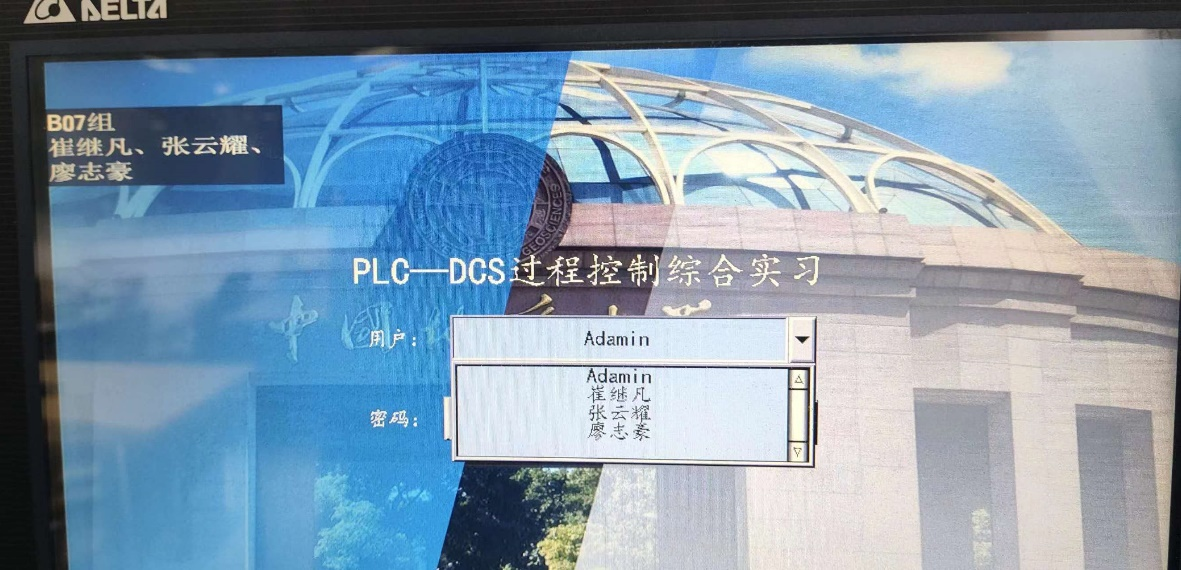
\includegraphics[width=0.8\textwidth]{figure/HMI登录界面实拍.png} 
    \caption{HMI登录界面实拍} % caption是图片的标题
    \label{fig:img5} % 此处的label相当于一个图片的专属标志,目的是方便上下文的引用
\end{figure}

%%%
\subsubsection{用户界面设计}
%%%%
\paragraph{图形化主界面}~{}

登录后,系统默认跳转到如图\ref{fig:img6}的图形化操作界面。界面左侧是系统的整体状态图,主要显示主水箱水位和大小两个水箱的水位,水箱一侧包含刻度,便于直接读取水箱液位情况。

界面右侧是四个显示仪表和三个操作界面。四个显示仪表显示系统部分主要传感器的参数。分别为小水箱开度,大水箱变频器,大水箱流量,流量压力。仪表下方还包括数值显示框,能够更精确的读取数值。
\begin{figure}[H]
    \centering % 居中 
    % 图片文件的相对路径
    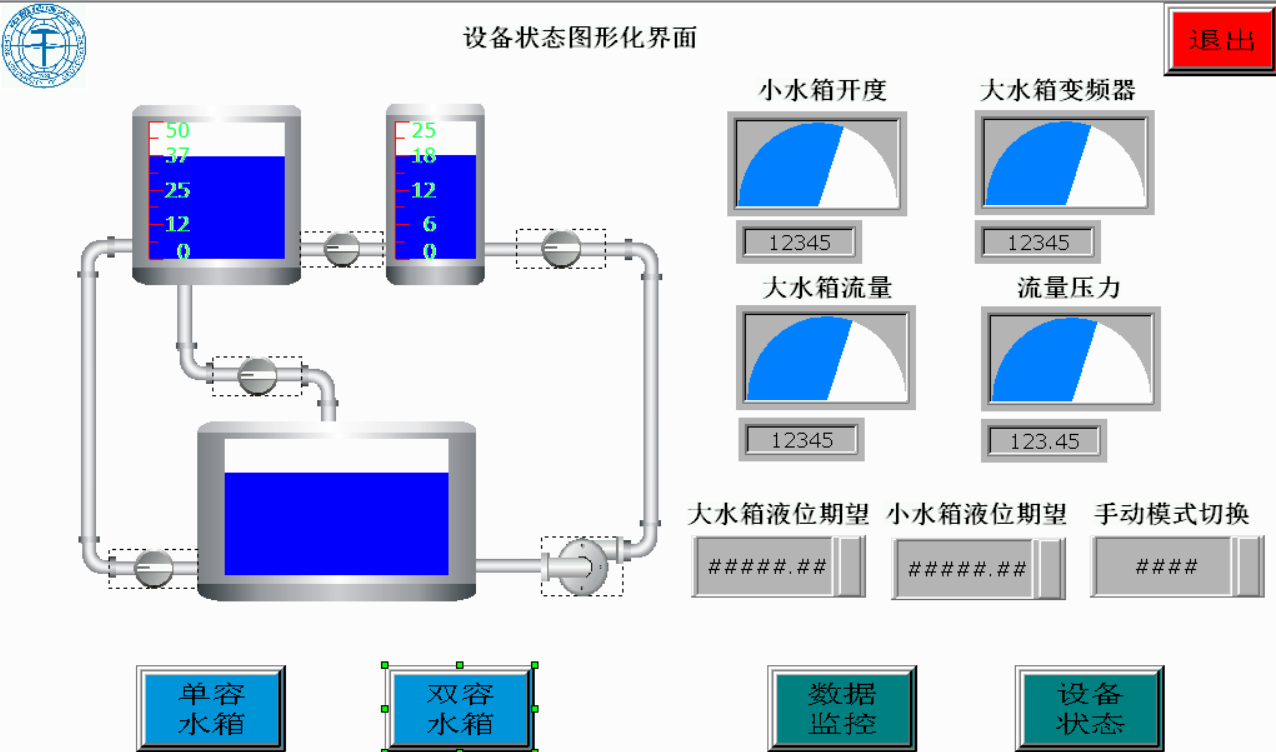
\includegraphics[width=0.8\textwidth]{figure/HMI图形化操作界面.png} 
    \caption{HMI图形化操作界面} % caption是图片的标题
    \label{fig:img6} % 此处的label相当于一个图片的专属标志,目的是方便上下文的引用
\end{figure}

图形化主界面下方是操作按键。左下方的分别为单容水箱操作界面切换按键,双容水箱操作界面切换按键。该蓝色按键访客不可按下,管理者与操作者可以按下。

右下方为数据监控界面切换按键与设备状态界面切换按键。如图\ref{fig:img6}所示的即为默认的设备状态图形化显示界面。而数据监控界面则是系统所有参数显示与设置的最高级菜单。该按键仅运行管理者按下并访问。

%%%%
\paragraph{单容水箱与双容水箱界面}~{}

如图\ref{fig:img7}所示单容水箱与双容水箱界面均主要由三个部分组成包括历史数据图,数据显示栏和控制切换输入/按键组成。左上方的三个图分别为大水箱实际液位,小水箱实际液位和大水箱流量。
\begin{figure}[H]
    \centering % 居中 
    % 图片文件的相对路径
    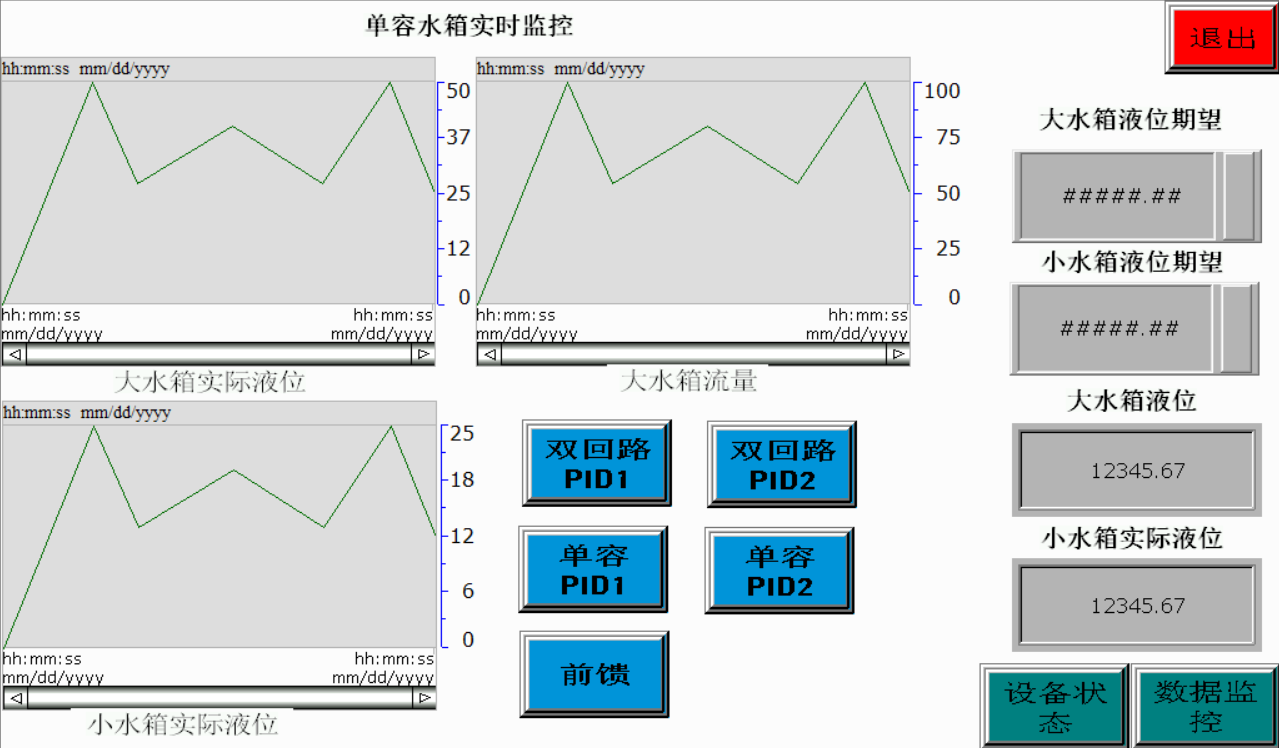
\includegraphics[width=0.8\textwidth]{figure/单容水箱监控操作界面.png} 
    \caption{单容水箱监控操作界面} % caption是图片的标题
    \label{fig:img7} % 此处的label相当于一个图片的专属标志,目的是方便上下文的引用
\end{figure}

如图\ref{fig:img8}所示,三个图表使用历史数据组件,设置采样周期为100ms,采样次数为300.即每采样300次形成一个数据点显示在图中,并根据这些采样点绘制时域变化的折线图。
\begin{figure}[H]
    \centering % 居中 
    % 图片文件的相对路径
    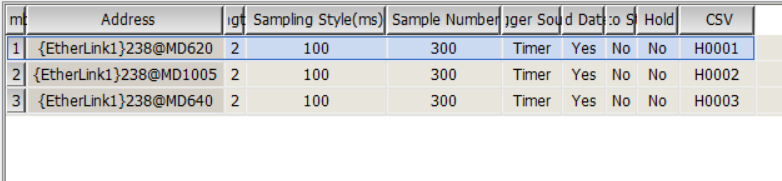
\includegraphics[width=0.8\textwidth]{figure/系统数据图标采样设置.png} 
    \caption{系统数据图标采样设置} % caption是图片的标题
    \label{fig:img8} % 此处的label相当于一个图片的专属标志,目的是方便上下文的引用
\end{figure}

系统界面中的蓝色按键则为控制方式的切换。如图\ref{fig:img7}所示。单容水箱系统,本次实习我们设计了五种控制方式,分别是单回路PID1,单回路PID2,双回路PID1,双回路PID2和前馈控制。这里的PID1和PID2分别使用西门子自带的PID控制模块和我们自己编写的PID控制程序。这么做是为了比较自行设计的PID控制器与自带的控制模块的控制性能差异。结果显示,自行设计的PID性能更好,调节实践更短,抗扰动能力更强。但PID模块使用上会更加方便快捷。

如图\ref{fig:img9},双容水箱与单容水箱类似。双容水箱、主要设计使用了比值和双容两种控制方式。
\begin{figure}[H]
    \centering % 居中 
    % 图片文件的相对路径
    \includegraphics[width=0.8\textwidth]{figure/双容水箱监控操作界面.png} 
    \caption{双容水箱监控操作界面} % caption是图片的标题
    \label{fig:img9} % 此处的label相当于一个图片的专属标志,目的是方便上下文的引用
\end{figure}

界面右侧则为大小水箱实际液位的显示框,可以更加精确的读取数值。右侧还包括大小水箱的液位期望设置栏,操作人员可以点击后,通过键盘输入期望的液位。

此外,界面中的三个图具有历史数据显示记录功能,可以通过拖动下方的滑动条来查看系统历史运行状况。图表右侧有显示刻度条,便于操作者通过历史数据点,读出系统历史运行数据。界面右下角的绿色按键可以返回设备状态界面。右上角的红色退出按键可以使系统立刻停止运行并退回到系统登录主界面。

%%%%
\paragraph{数据监控界面}~{}

如图\ref{fig:img10}所示为系统设备详细参数设置界面。该界面为系统最高权限界面,只有以系统管理者身份登录时才有权访问。该界面可以直接查看几乎所有系统传感器的数值。并可以对系统所有可调整参数进行设置。界面中,蓝色按键可以直接切换系统运行状态。此外还可以通过模式切换选框手动切换系统运行模式。手动模式切换中还包括处正常装态外的检修运行模式,测量运行模式等模式。极大的方便了操作者使用管理系统。
\begin{figure}[H]
    \centering % 居中 
    % 图片文件的相对路径
    \includegraphics[width=0.8\textwidth]{figure/数据监控界面.png} 
    \caption{数据监控界面} % caption是图片的标题
    \label{fig:img10} % 此处的label相当于一个图片的专属标志,目的是方便上下文的引用
\end{figure}

%%%
\subsubsection{系统运行实例}
如图\ref{fig:img11}和图\ref{fig:img12}所示为系统在运行检修模式时的情形,此时所有水箱均为空,各传感器数值为0,系统处于待工作状态。
\begin{figure}[H]
    \centering % 居中 
    % 图片文件的相对路径
    \includegraphics[width=0.8\textwidth]{figure/设备运行状态界面(待工作状态).png} 
    \caption{设备运行状态界面(待工作状态)} % caption是图片的标题
    \label{fig:img11} % 此处的label相当于一个图片的专属标志,目的是方便上下文的引用
\end{figure}
\begin{figure}[H]
    \centering % 居中 
    % 图片文件的相对路径
    \includegraphics[width=0.8\textwidth]{figure/单容水箱运行状态界面(待工作状态).png} 
    \caption{单容水箱运行状态界面(待工作状态)} % caption是图片的标题
    \label{fig:img12} % 此处的label相当于一个图片的专属标志,目的是方便上下文的引用
\end{figure}

如图\ref{fig:img13}为系统正常运行状态界面,对于不同数据要求不同,固显示精度存在差异,一般为整数型或精确到小数点后两位。
\begin{figure}[H]
    \centering % 居中 
    % 图片文件的相对路径
    \includegraphics[width=0.8\textwidth]{figure/系统正常运行状态界面.png} 
    \caption{系统正常运行状态界面} % caption是图片的标题
    \label{fig:img13} % 此处的label相当于一个图片的专属标志,目的是方便上下文的引用
\end{figure}

%%
\subsection{数据处理与转换}
PLC与HMI之间建立TCP可靠连接来进行数据通讯。HMI想要读取或写入时需要访问PLC内的内存地址。如图\ref{fig:img14},需要设置屏幕读入的接口和对应PLC的内存地址。读写分离设置,同时如果有必要还需要设置读写地址的偏移量,以保证数据的正确。
\begin{figure}[H]
    \centering % 居中 
    % 图片文件的相对路径
    \includegraphics[width=0.6\textwidth]{figure/读写地址设置.png} 
    \caption{读写地址设置} % caption是图片的标题
    \label{fig:img14} % 此处的label相当于一个图片的专属标志,目的是方便上下文的引用
\end{figure}

本次实习所使用的西门子S7 1200PLC控制器主要实用的数据类型包括Bool、Byte、Word、Dword、Int、Dint和Real等。待HMI将数据读取后需要显示数据。而对于显示数据的设置如图\ref{fig:img15}、图\ref{fig:img16}所示。首先需要设置数据类型,显示数据为一字(Word)或双字(Word),部分数据格式必须需用双字如浮点型(Floating)等。
\begin{figure}[H]
    \centering % 居中 
    % 图片文件的相对路径
    \includegraphics[width=0.6\textwidth]{figure/数据类型设置14.png} 
    \caption{数据类型设置} % caption是图片的标题
    \label{fig:img15} % 此处的label相当于一个图片的专属标志,目的是方便上下文的引用
\end{figure}
\begin{figure}[H]
    \centering % 居中 
    % 图片文件的相对路径
    \includegraphics[width=0.6\textwidth]{figure/数据类型设置15.png} 
    \caption{数据类型设置} % caption是图片的标题
    \label{fig:img16} % 此处的label相当于一个图片的专属标志,目的是方便上下文的引用
\end{figure}

数据类型设置主要包括BCD码,十六进制数(HEX),二进制数(Binary),浮点数(Floating)等。在使用这些数据时应当注意PLC与HMI之间有时需要进行数据转换和对应。查询台达官网可得到如图\ref{fig:img17}的寄存器使用表。
\begin{figure}[H]
    \centering % 居中 
    % 图片文件的相对路径
    \includegraphics[width=0.8\textwidth]{figure/寄存器数据类型.png} 
    \caption{寄存器数据类型} % caption是图片的标题
    \label{fig:img17} % 此处的label相当于一个图片的专属标志,目的是方便上下文的引用
\end{figure}

此外,显示一般还需要设置显示精度,这里我们对于浮点数统一设置为5位整数和两位小数。

%%
\subsection{编译与下载}
在编译下载之前,需要首先进行下载的配置。在“选项”栏中,点击进入“环境设置”这一选项。可选择上/下载设置是通过 USB 直接连接还是以太网路连接。本次实习通过有线网络与HMI进行通讯,因此勾选“以太网路”即可。

当所有内容设计完成后,需要把内容编译后传入HMI内。固首先点击设计栏的工具选项->全部编译。软件会自动编译已经设计完成的界面。当设计存在问题,如大小不匹配,输入地址为空等问题时,发生报错并指向错误发生的位置。

编译完成后点击设计栏的工具选项,点击下载全部资料会进入位址选择界面。我们首先要将电脑与屏幕链接的端口的IPV4的IP地址设置在与屏幕IP地址同一子网下且不冲突。

此处设置为192.168.1.200,子网掩码为默认的255.255.255.0。这是通过自动搜索我们就可以找到对应的HMI。单击HMI选项后点击传输开始,等待程序自动完成上传后就可以在屏幕端与PLC建立起链接,实现图形化数据显示与控制调整。
\begin{figure}[H]
    \centering % 居中 
    % 图片文件的相对路径
    \includegraphics[width=0.8\textwidth]{figure/位低选择.png} 
    \caption{位地选择} % caption是图片的标题
    \label{fig:img18} % 此处的label相当于一个图片的专属标志,目的是方便上下文的引用
\end{figure}

此外为了保证PLC与HMI之间正常的数据通讯还需要HMI与PLC正确建立链接。除了上述所说填写正确的Controller IP地址还需要在博图软件中对PLC正确设置。

如图\ref{fig:img19}设置PLC的静态IP地址:
\begin{figure}[H]
    \centering % 居中 
    % 图片文件的相对路径
    \includegraphics[width=0.8\textwidth]{figure/PLC地址设置.png} 
    \caption{PLC地址设置} % caption是图片的标题
    \label{fig:img19} % 此处的label相当于一个图片的专属标志,目的是方便上下文的引用
\end{figure}

设置后点击选项-常规-防护与安全中的链接机制,勾选允许来自远程对象的PUTIGET通讯访问。否则HMI无法正确与PLC建立TCP连接并报错。
\begin{figure}[H]
    \centering % 居中 
    % 图片文件的相对路径
    \includegraphics[width=0.8\textwidth]{figure/PLC访问控制.png} 
    \caption{PLC访问控制} % caption是图片的标题
    \label{fig:img20} % 此处的label相当于一个图片的专属标志,目的是方便上下文的引用
\end{figure}

此外为了检测数据的正确通讯,建立通讯程序块,并设置对应的端口与连接类型。如图\ref{fig:img21}所示。
\begin{figure}[H]
    \centering % 居中 
    % 图片文件的相对路径
    \includegraphics[width=0.8\textwidth]{figure/通讯程序块.png} 
    \caption{通讯程序块} % caption是图片的标题
    \label{fig:img21} % 此处的label相当于一个图片的专属标志,目的是方便上下文的引用
\end{figure}

最后,在数据通讯程序块中关闭“优化的块访问”。该功能可能导致数据通讯异常。如图\ref{fig:img22}所示。
\begin{figure}[H]
    \centering % 居中 
    % 图片文件的相对路径
    \includegraphics[width=0.8\textwidth]{figure/关闭块优化访问.png} 
    \caption{关闭块优化访问} % caption是图片的标题
    \label{fig:img22} % 此处的label相当于一个图片的专属标志,目的是方便上下文的引用
\end{figure}

%
\section{实习心得与体会}

在实习的过程中,我们遇到过很多问题。比如刚开始调试程序时发现变频泵动不了,液位计读出的数据与实际不一致等等,后来经老师提醒才发现水箱设备与PLC的接线并不一定与实验指导书给出的一致。出现这个问题,一部分原因在于我们对PLC的工作方式还不是特别熟悉,其实了解了以后就会发现它和单片机的工作方式差不多。具体到接线这个问题上,无非就是需要弄清楚PLC有哪些类型的输入输出接口,这些接口在PLC中对应的地址是多少,以及各种传感器和执行器的信号和这些接口是如何对应的。经过一些观察和尝试,很容易就可以把这些地址修改成正确的对应关系。

我们实习的过程中花了很大一部分精力在计算机和PLC之间的网络通信上,比如虚拟机的网络通道配置问题,以及在网络通信没有问题的情况下可能还会出现其他问题,比如PLC无法访问、设备组态错误等等。面对这些问题我的心得是,首先不要有畏难情绪,而要一个问题一个问题地找到解决方法,而且在问题得到解决以后最好把解决方法记录下来。我在实习的时候就详细记录了虚拟机网络配置过程的截图,以防之后需要配置网络时忘记具体步骤。之所以要这样做,还有一部分原因在于难免会有一些同学对设备还不太熟悉,操作这些设备的方式可能不一定正确,导致我们再使用时又会发现设备出现了这样那样的小问题。记得有一段时间我们去实习的第一步就是把网络通信、设备组态重新配置一遍,有时候排查问题需要花很多时间。我印象很深的一次是某天晚上我们花了好几个小时的时间来解决设备的通信错误,直到已经很晚了我们也没能解决问题,不得不离开实验室,这件事也导致我们不得不选择临时更换设备,耽误了很多时间。总而言之,对遇到的问题,及时记录下解决方案是非常有必要的。

针对遇到的这些问题的解决方法,还有很重要的一点是要充分利用好自己手中的资源,比如网络上的资源,包括同学、老师和助教,都是我们获取解决问题的新思路、新知识和新技能的重要来源,简单来说就是要积极的和身边的人多交流。此外还有一些需要注意的细节,在对设备组态进行配置时最好一步一步认真对照,比如不同类型接口的数量要弄清楚,以防配置的时候出现遗漏,以及信号的类型是电流还是电压、信号的范围是多少等等。在解决这些问题的过程中,我们小组各成员之间的协调合作也得到了加强。通过所有成员的共同努力,最终设计出一个满意的作品,这个过程是非常令人有成就感的。

总的来说,通过这次实习,我学到了很多新的知识和技能,也锻炼了自己解决问题的能力,吸取了教训,也积累了很多经验,希望以后可以有机会将这些技能应用到解决生活中实际问题上,也在此衷心感谢这段时间里两位老师和助教学长的帮助和付出。

\end{document}